
\subsection{User behavior based layer preconstruction cache}
\label{sec:cache-design}

In the following, we present our \sysname~\preconstructcachename design.

%Each \texttt{pull layer} request has a precedent \texttt{pull manifest} request.
%Upon receiving a \texttt{pull manifest} request, 
%\sysname~sends the updated \sysname~manifest to client.
%After receiving a \sysname~manifest, the client parses the manifest
%and sends either a \texttt{pull layer} request if the layer hasn't been deduplicated,
%or a list of \texttt{pull slice} requests if a list of corresponding slices presents in the manifest.
%Those \texttt{pull slice} requests will then be
%forwarded to all the registry servers that store the requested
%layer's slices as shown in Figure~\ref{fig:sys-overview}. 

%\begin{figure*}[t]
%		\begin{minipage}{0.32\linewidth}
%			\centering
%			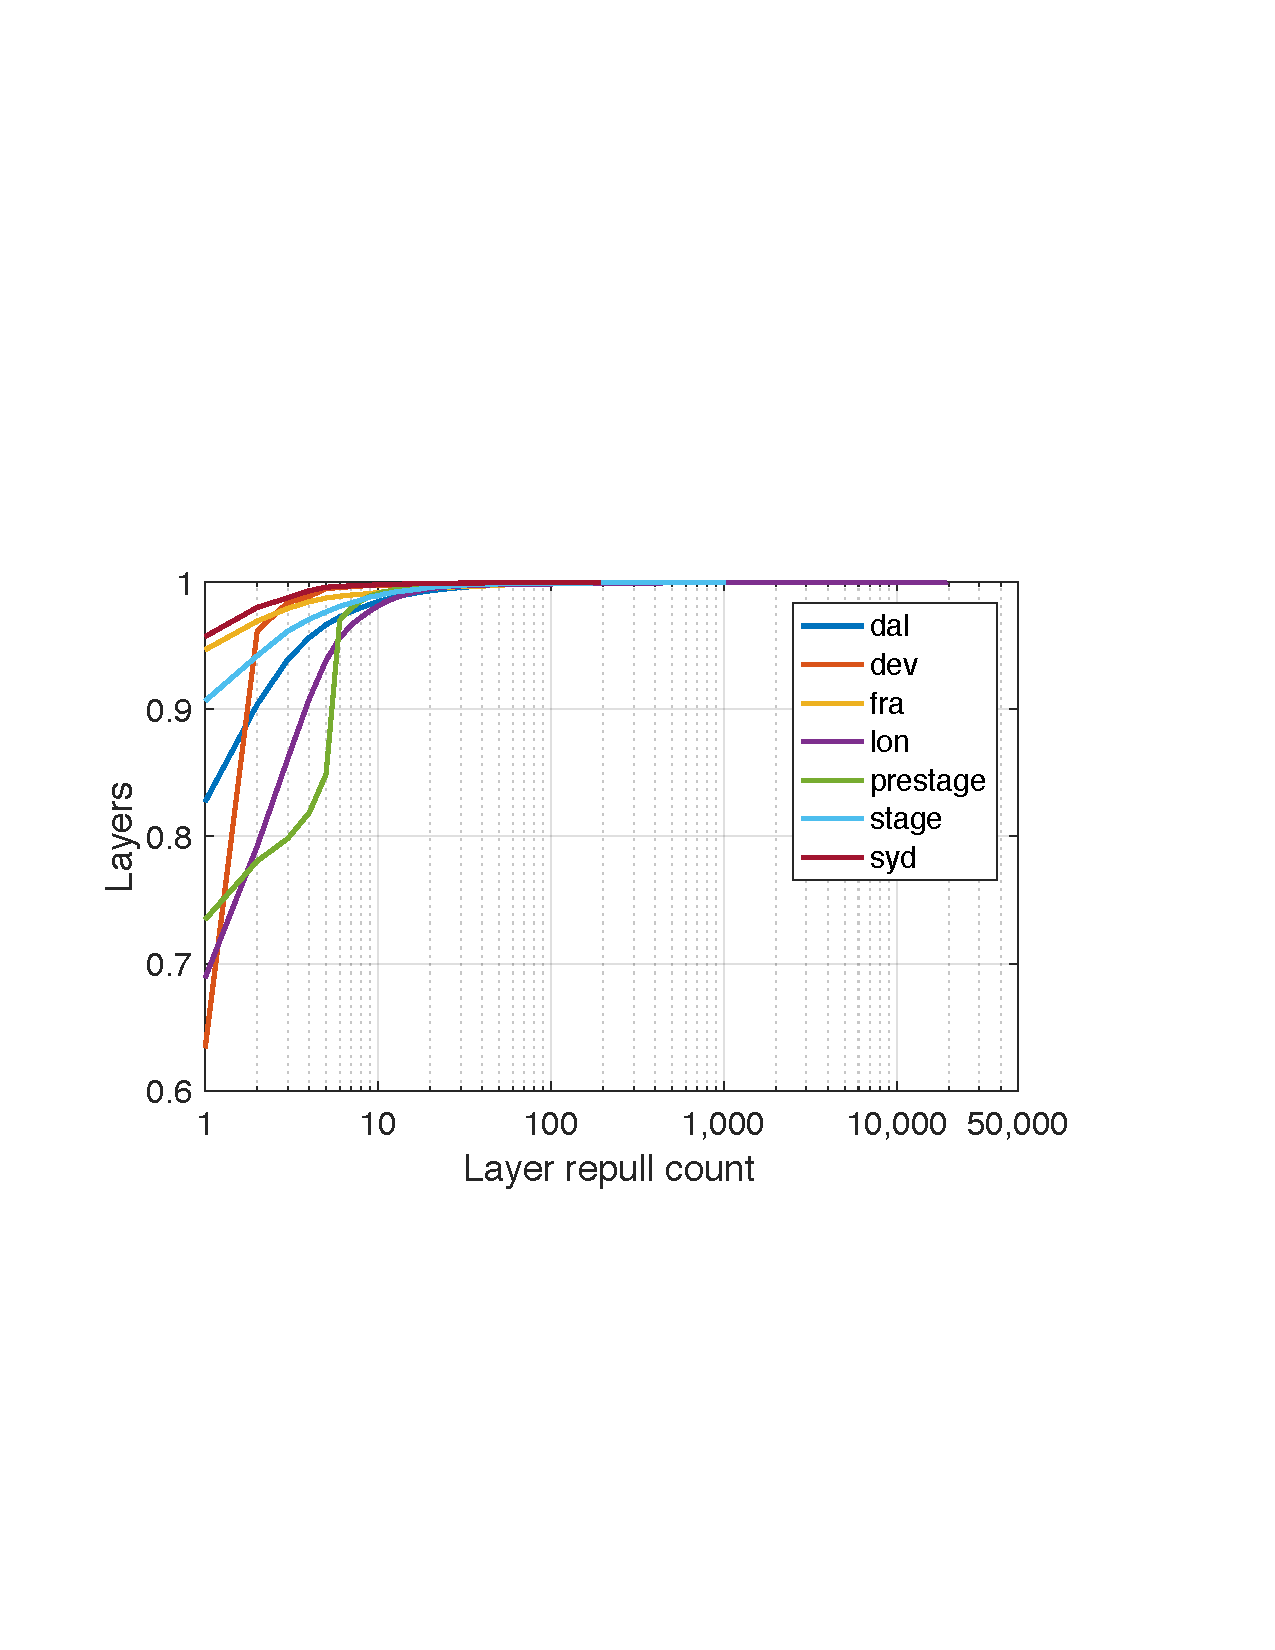
\includegraphics[width=1\textwidth]{graphs/cdf-layer-repull-by-same-client.pdf}
%			%\caption{CDF of layer repull count.}
%		%	\vspace{-3pt}
%			\label{fig:layer-repull-cdf}
%		\end{minipage}
%			\begin{minipage}{0.32\linewidth}
%				\centering
%				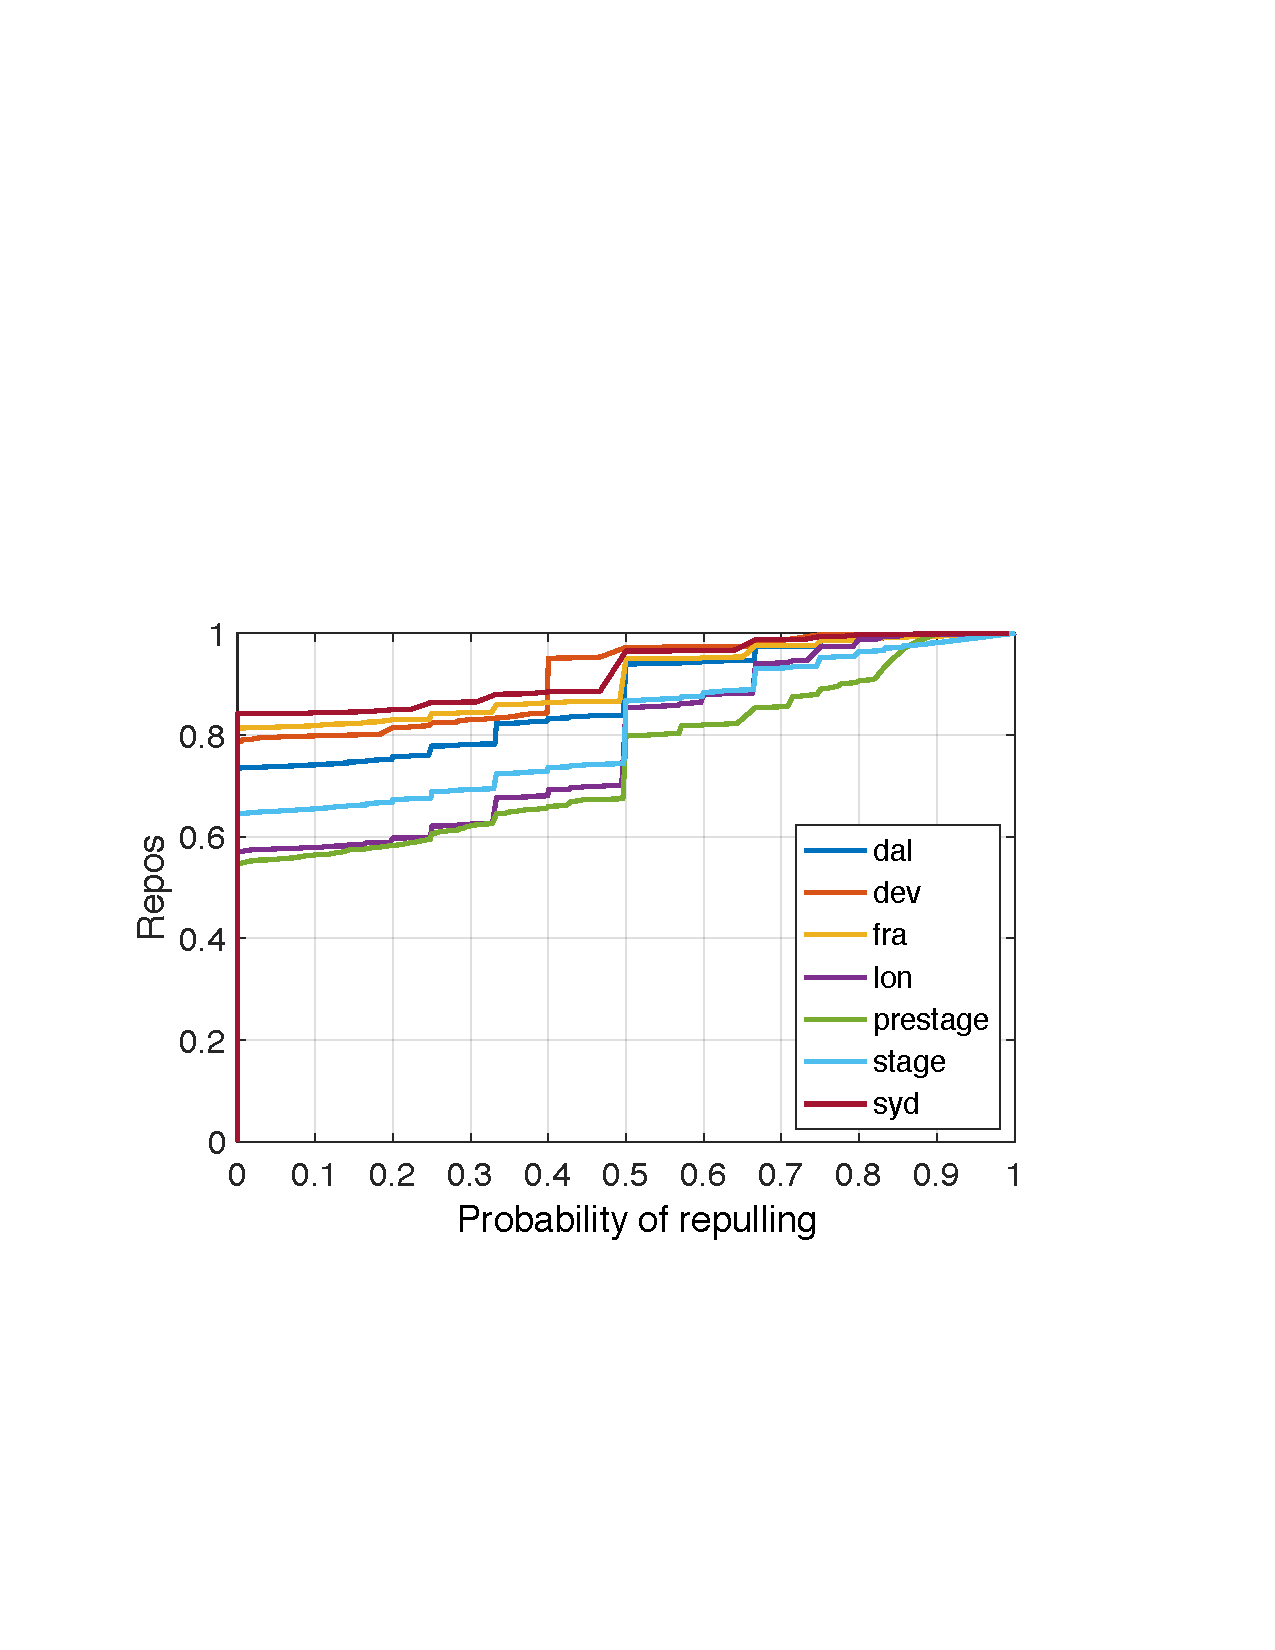
\includegraphics[width=1\textwidth]{graphs/cdf-repo-repull-ratio-by-same-client.pdf}
%				%\caption{PDF of repository repulling probability.}
%				%	\vspace{-3pt}
%				\label{fig:repo-repull-cdf}
%			\end{minipage}
%		\begin{minipage}{0.32\linewidth}
%			\centering
%			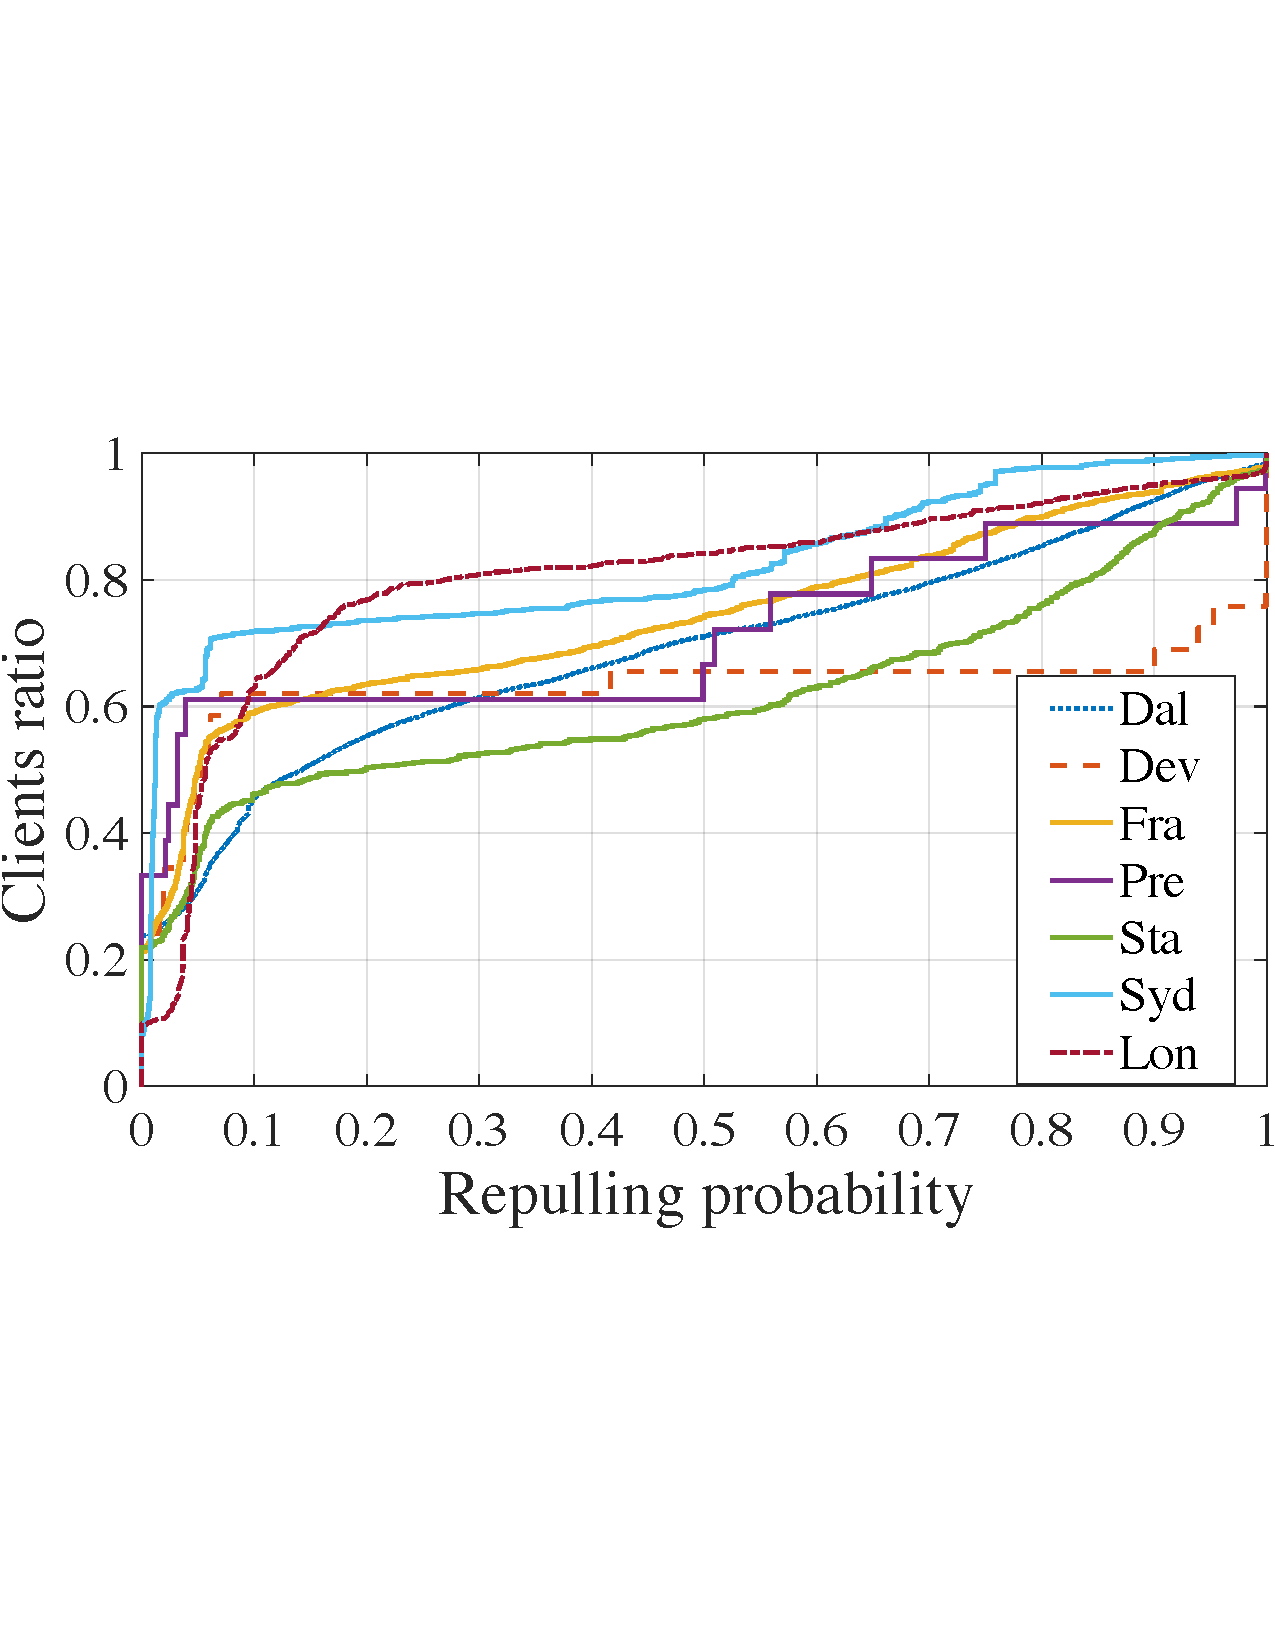
\includegraphics[width=1\textwidth]{graphs/cdf-client-repull-layer-request-ratio.pdf}
%			%
%			%	\vspace{-3pt}
%			\label{fig:client-repull-cdf}
%		\end{minipage}
%	\caption{PDF of client repull count, repository repulling probability, and client repulling probability..}
%\end{figure*}

%\begin{figure}[!t]
%	\centering
%	\subfigure[\texttt{GET} layer request count]{
%		\includegraphics[width=0.22\textwidth]{graphs/cdf-layer-repull-ratio-by-same-client.pdf}
%		\label{fig:layer-repull-cdf}
%	}
%%	\subfigure[Repository repulling probability]{
%%		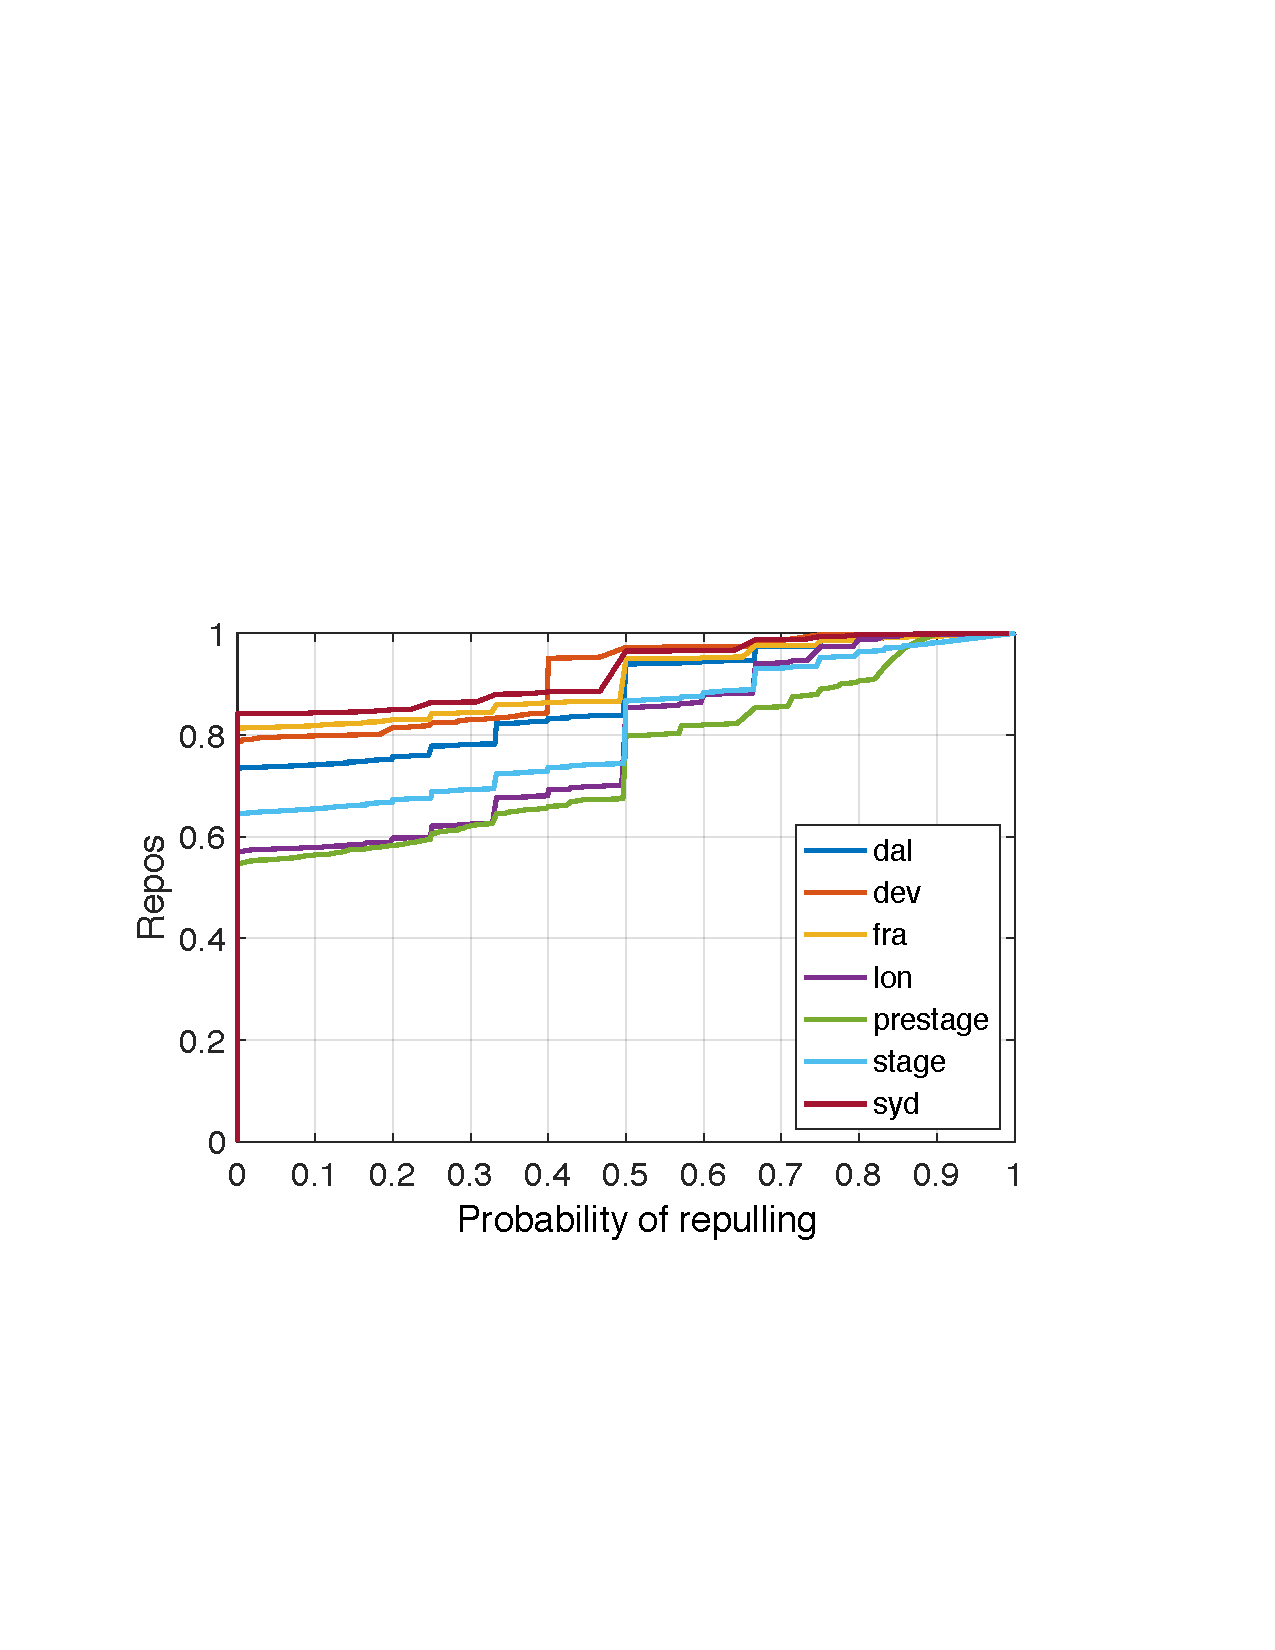
\includegraphics[width=0.2\linewidth]{graphs/cdf-repo-repull-ratio-by-same-client.pdf}
%%		\label{fig:repo-repull-cdf}
%%	}
%	\subfigure[Client repulling probability]{
%	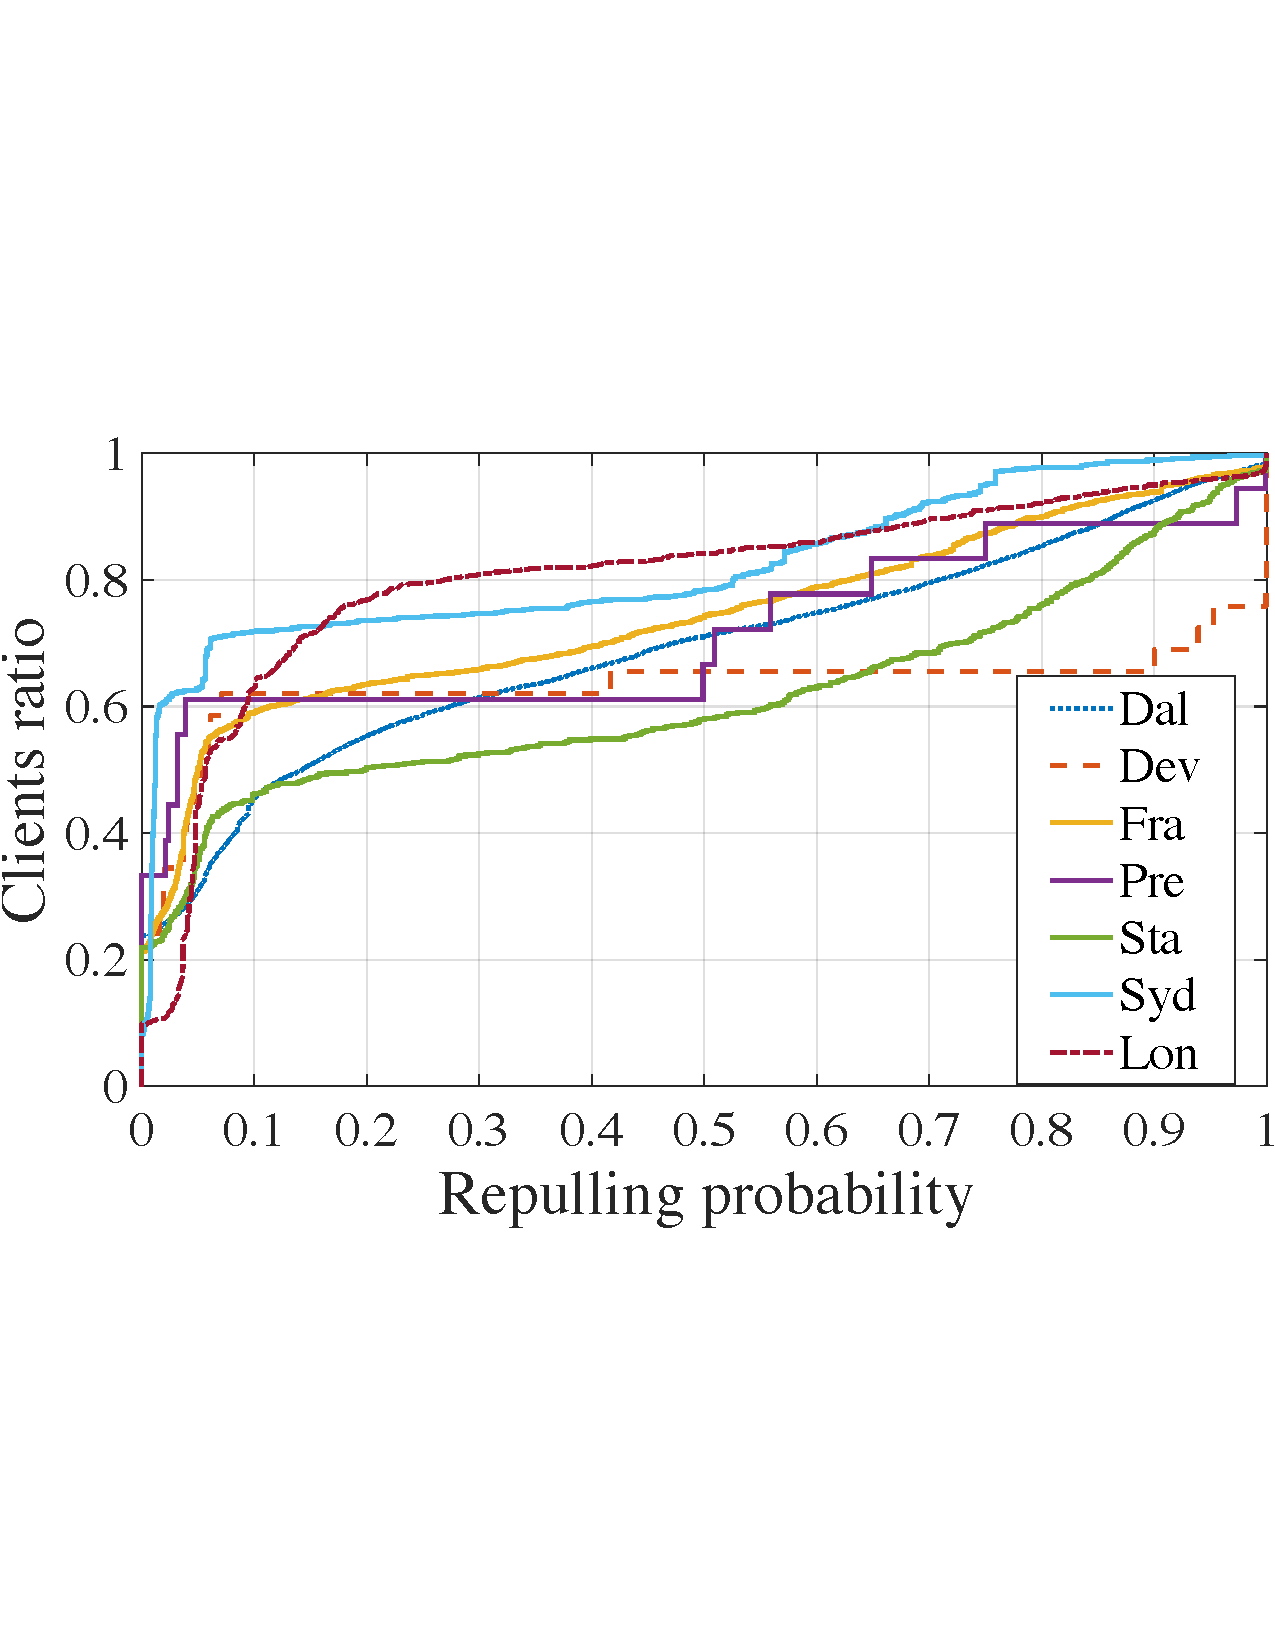
\includegraphics[width=0.2\textwidth]{graphs/cdf-client-repull-layer-request-ratio.pdf}
%   \label{fig:client-repull-cdf}
%}
%	\caption{CDF of \texttt{GET} layer request count and client repulling probability.}
%	\label{fig-repull}
%\end{figure}
%






\begin{figure*}[t]
        \centering
        \begin{minipage}{0.3\textwidth}
                \centering
                \includegraphics[width=0.9\textwidth]{{graphs/cdf-layer-repull-ratio-by-same-client.pdf}
                \caption{CDF of \texttt{GET} layer request count}
                \label{fig:layer-repull-cdf}
        \end{minipage}%
        \begin{minipage}{0.3\textwidth}
                \centering
                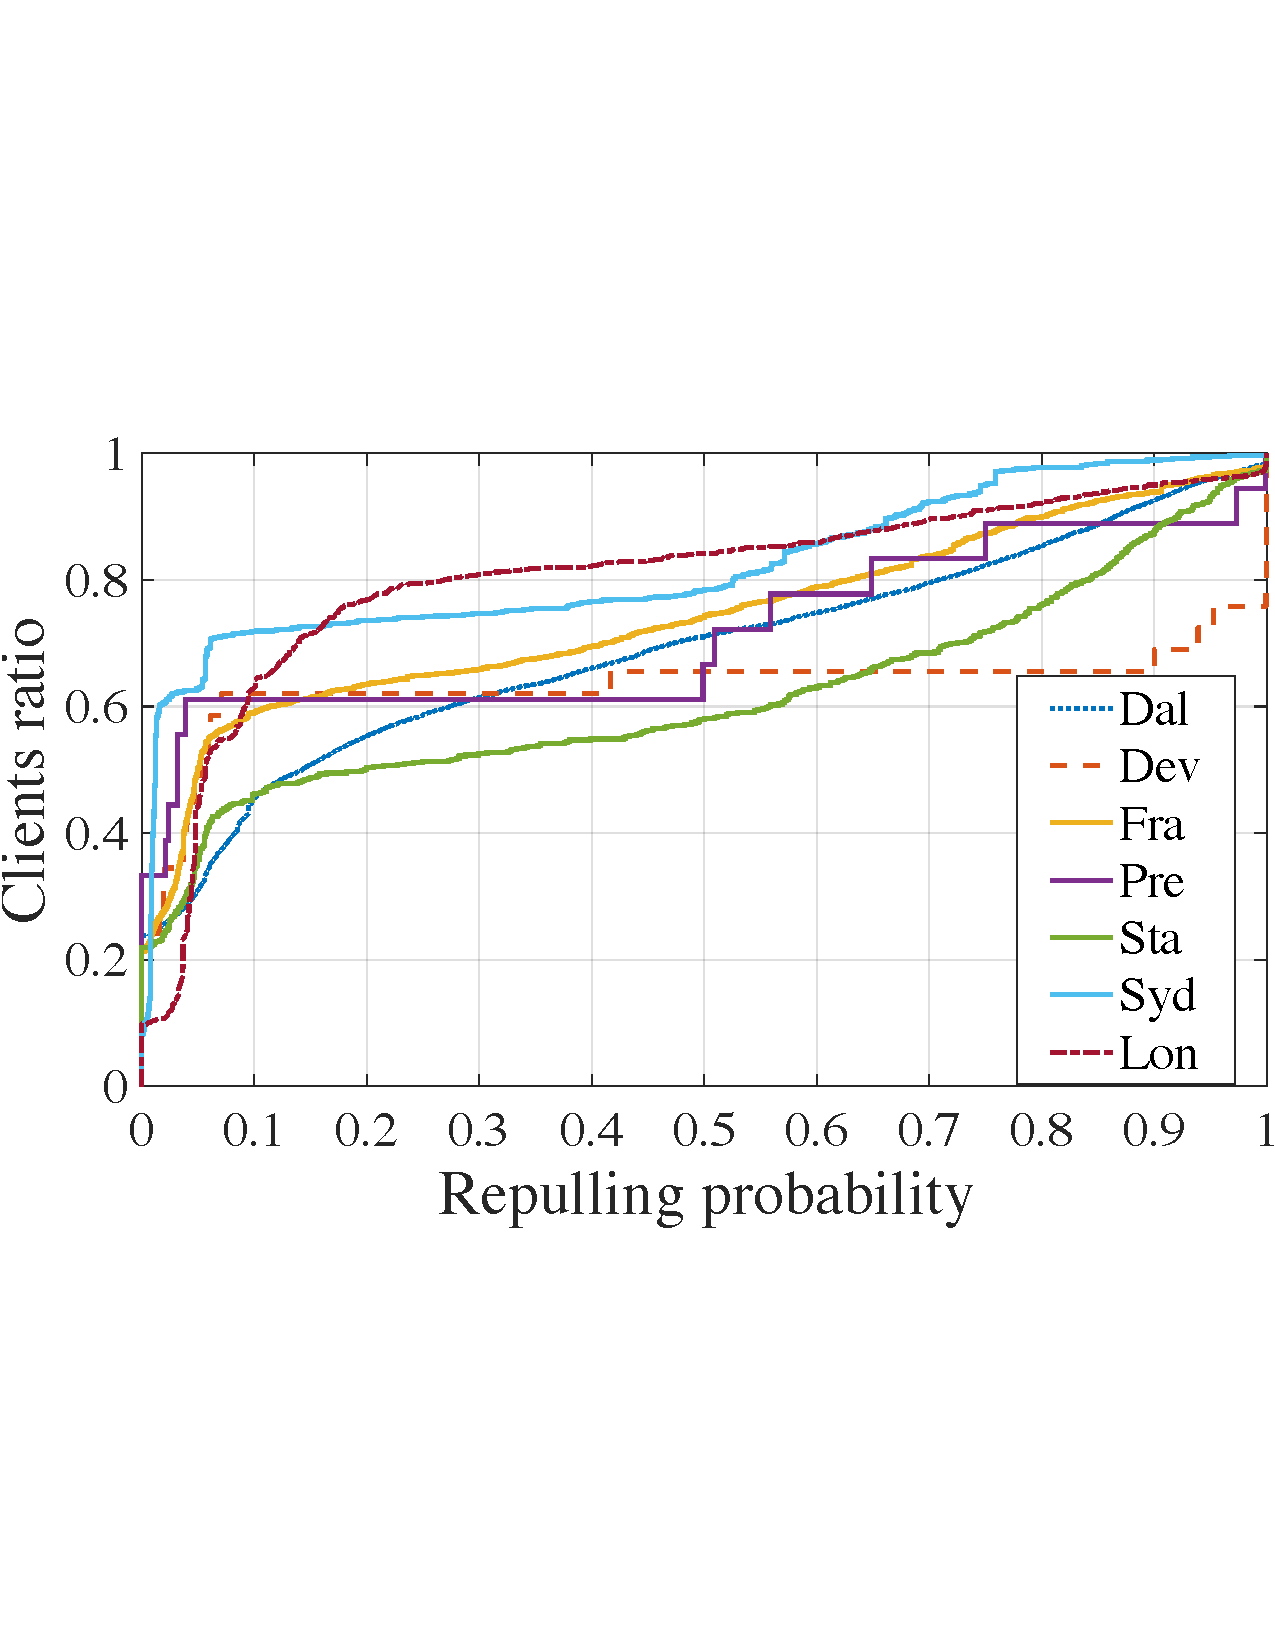
\includegraphics[width=0.9\textwidth]{graphs/cdf-client-repull-layer-request-ratio.pdf}
                \caption{CDF of Client repulling probability}% of LRU cache and preconstruct cache.}
                \label{fig:client-repull-cdf}
        \end{minipage}%
        \begin{minipage}{0.3\textwidth}
        \centering
        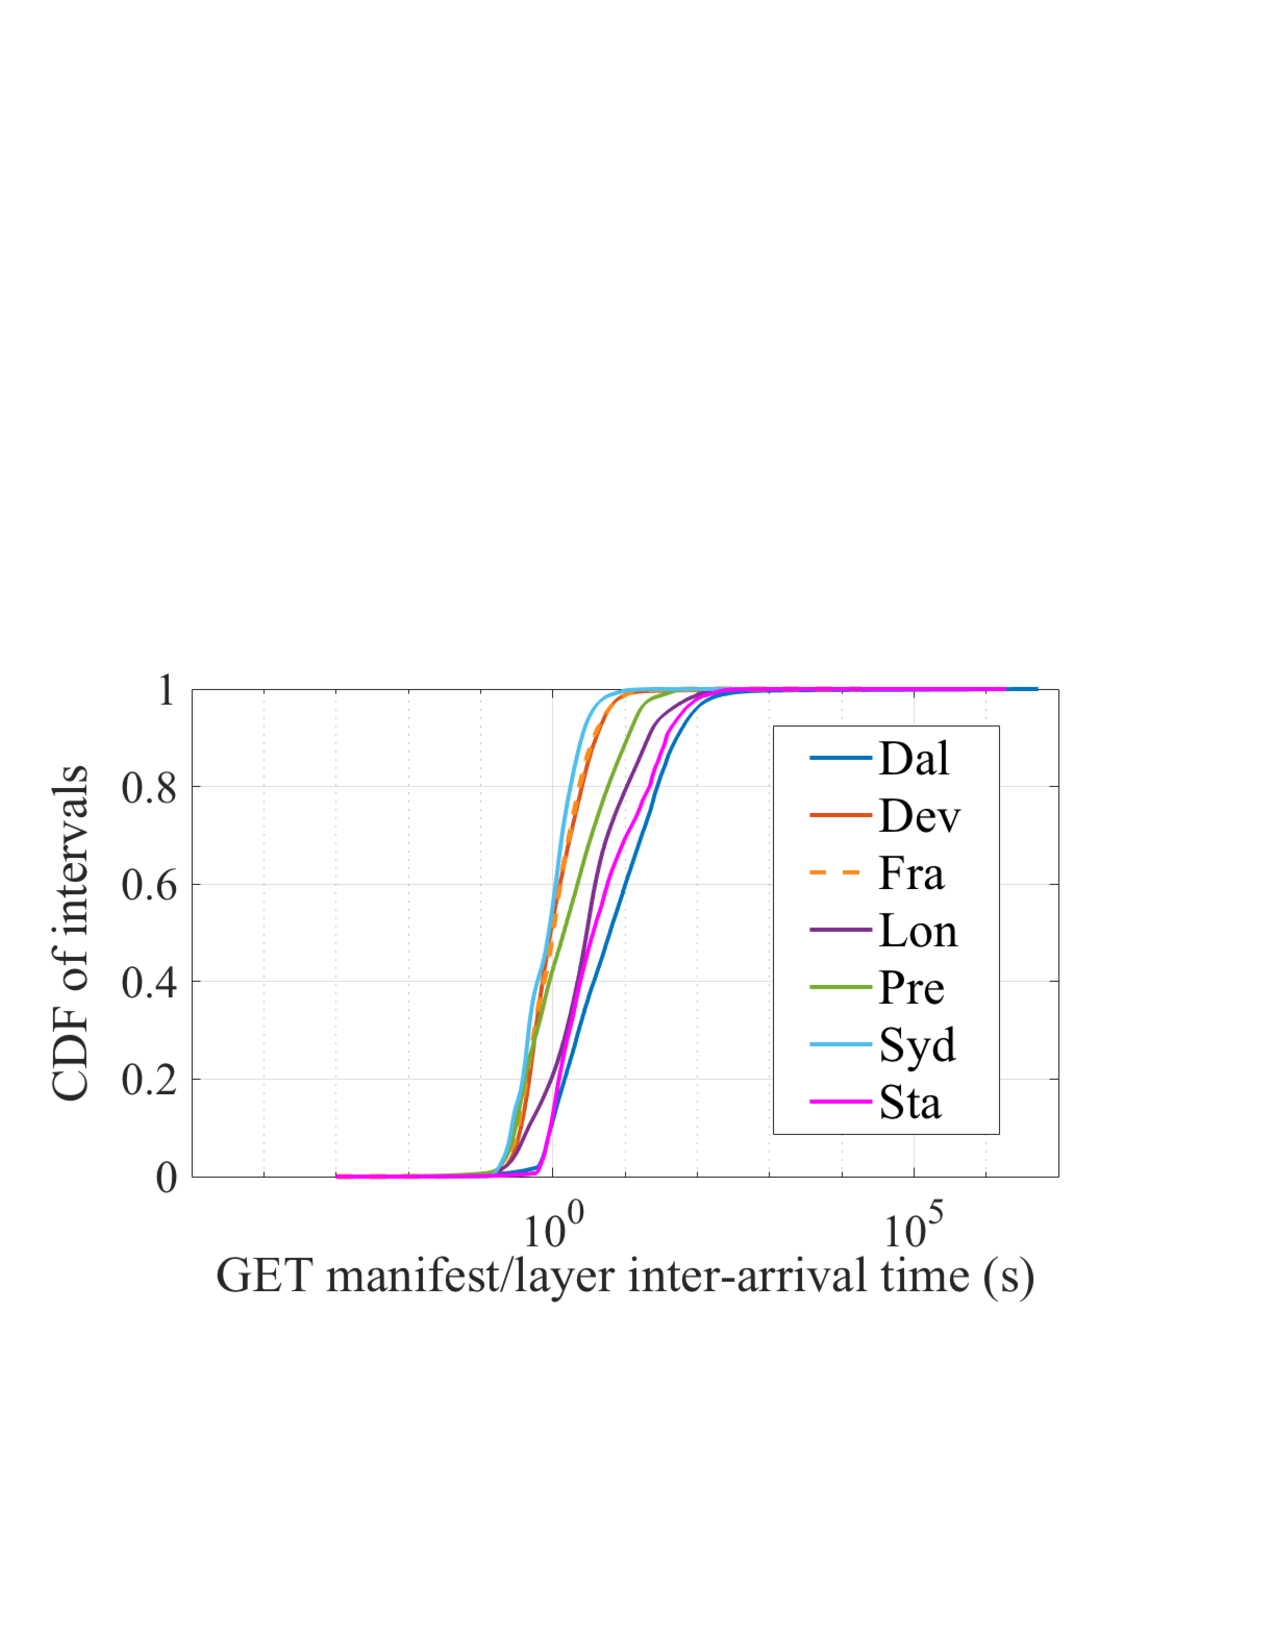
\includegraphics[width=0.9\textwidth]{graphs/GML-intervals.pdf}
        \caption{Intervals between \texttt{GET} manifest request and \texttt{GET} layer request}
        \label{fig:intervals}
   \end{minipage}
\end{figure*}





%\begin{figure}[!t]
%	\centering
%	\subfigure[CDF of compression ratio]{\label{fig_cdf_compression_ratio}
%		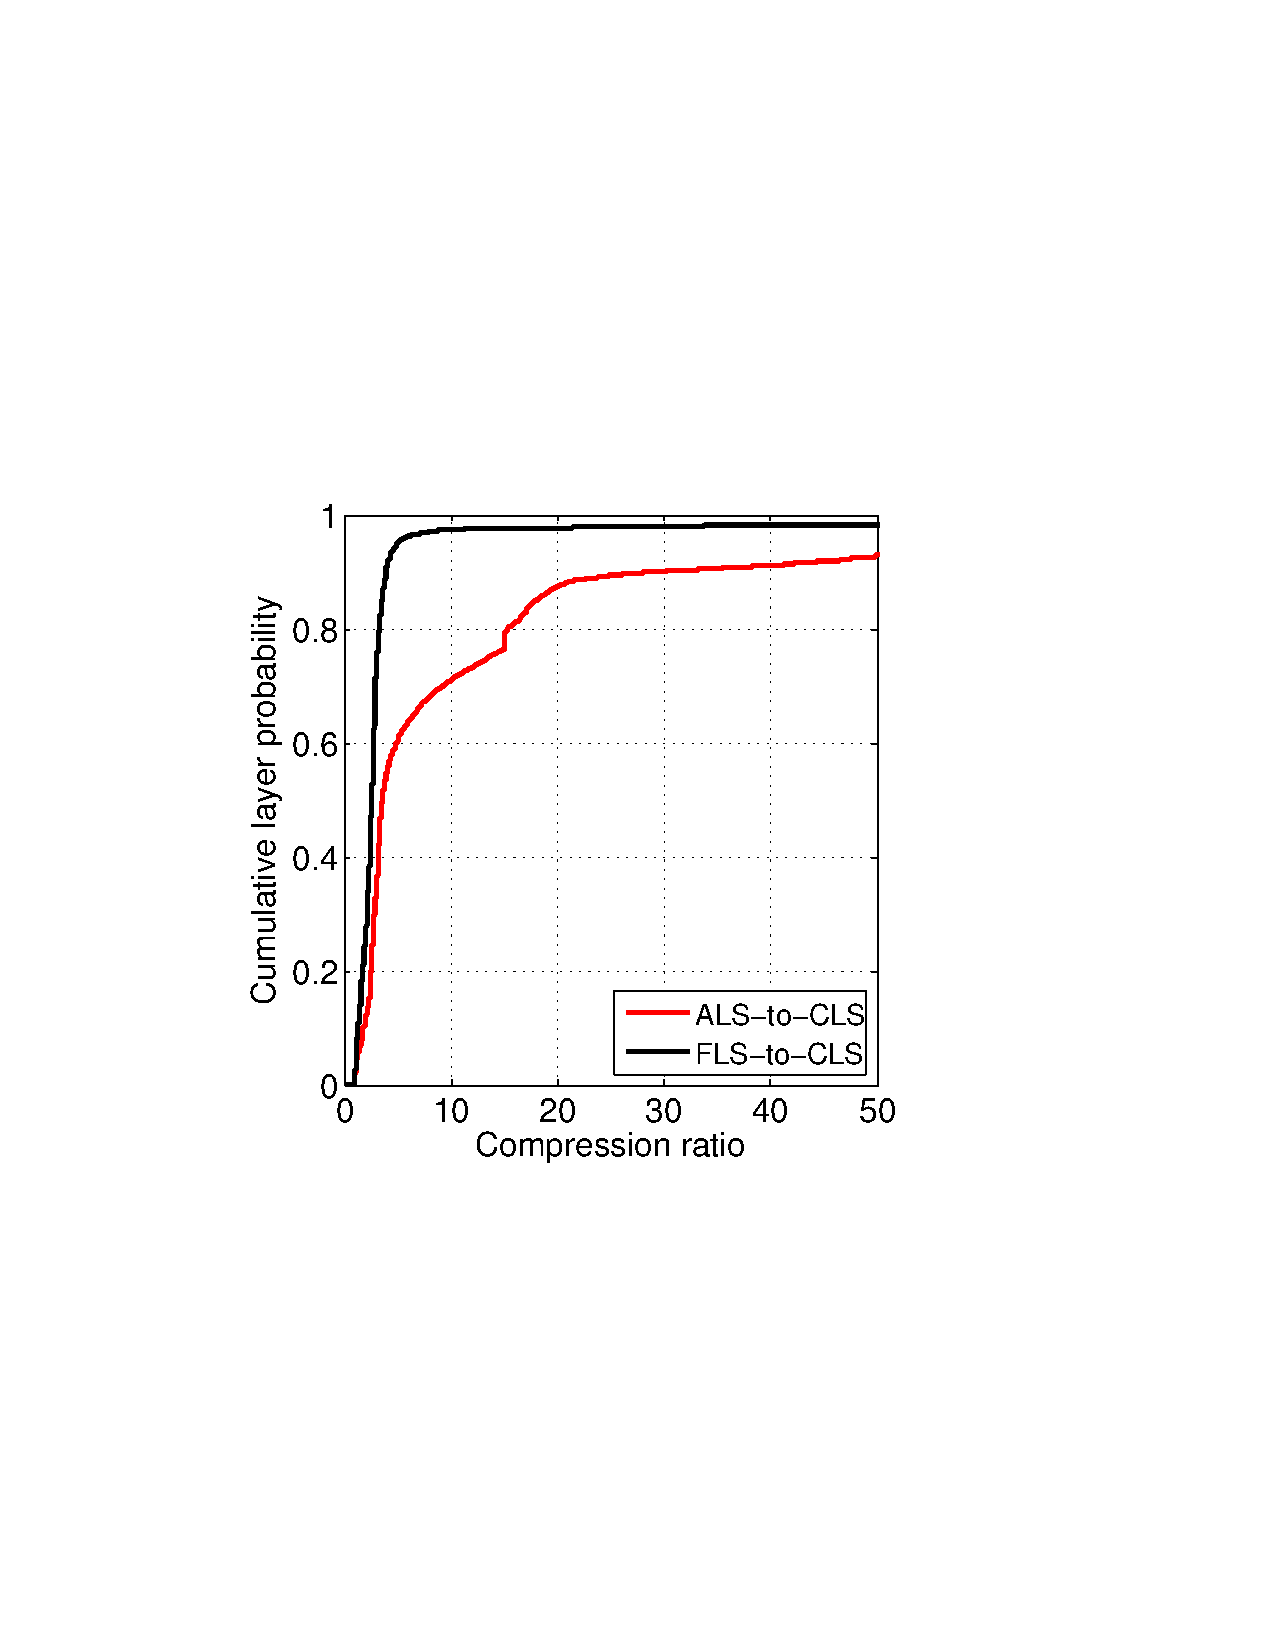
\includegraphics[width=0.23\textwidth]{graphs/cdf_compression_ratio.pdf}
%	}
%	\subfigure[Histogram of comp. ratios]{\label{fig_his_compression_ratio}
%		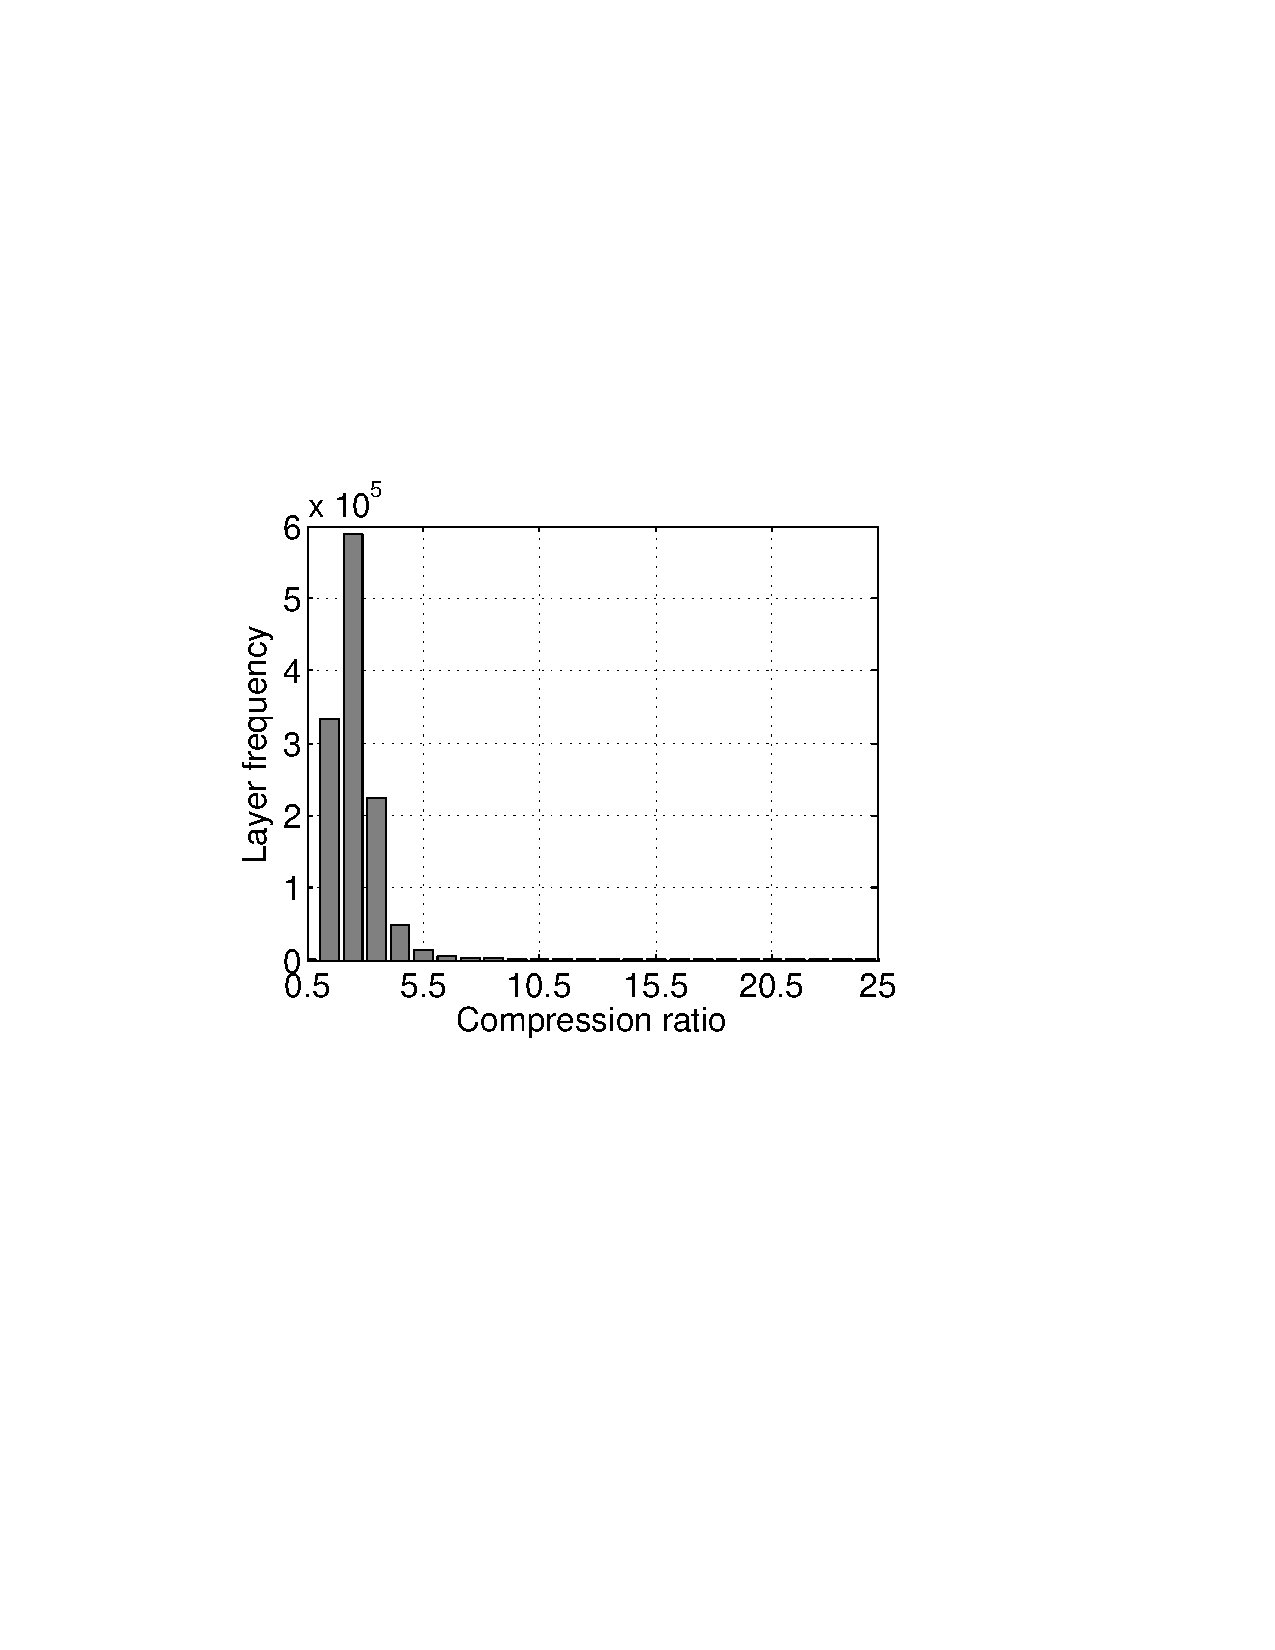
\includegraphics[width=0.223\textwidth]{graphs/his_compression_ratio.pdf}
%	}
%	\caption{Layer compression ratio distribution
%		%\vcomment{Different colors are used in figure (a) and (b) FLS/CLS\nancomment{will address later}}
%	}
%	\label{fig-compression-ratio}
%\end{figure}


%\begin{figure}[t]
%	\centering
%	\begin{minipage}{0.26\textwidth}
%		\centering
%		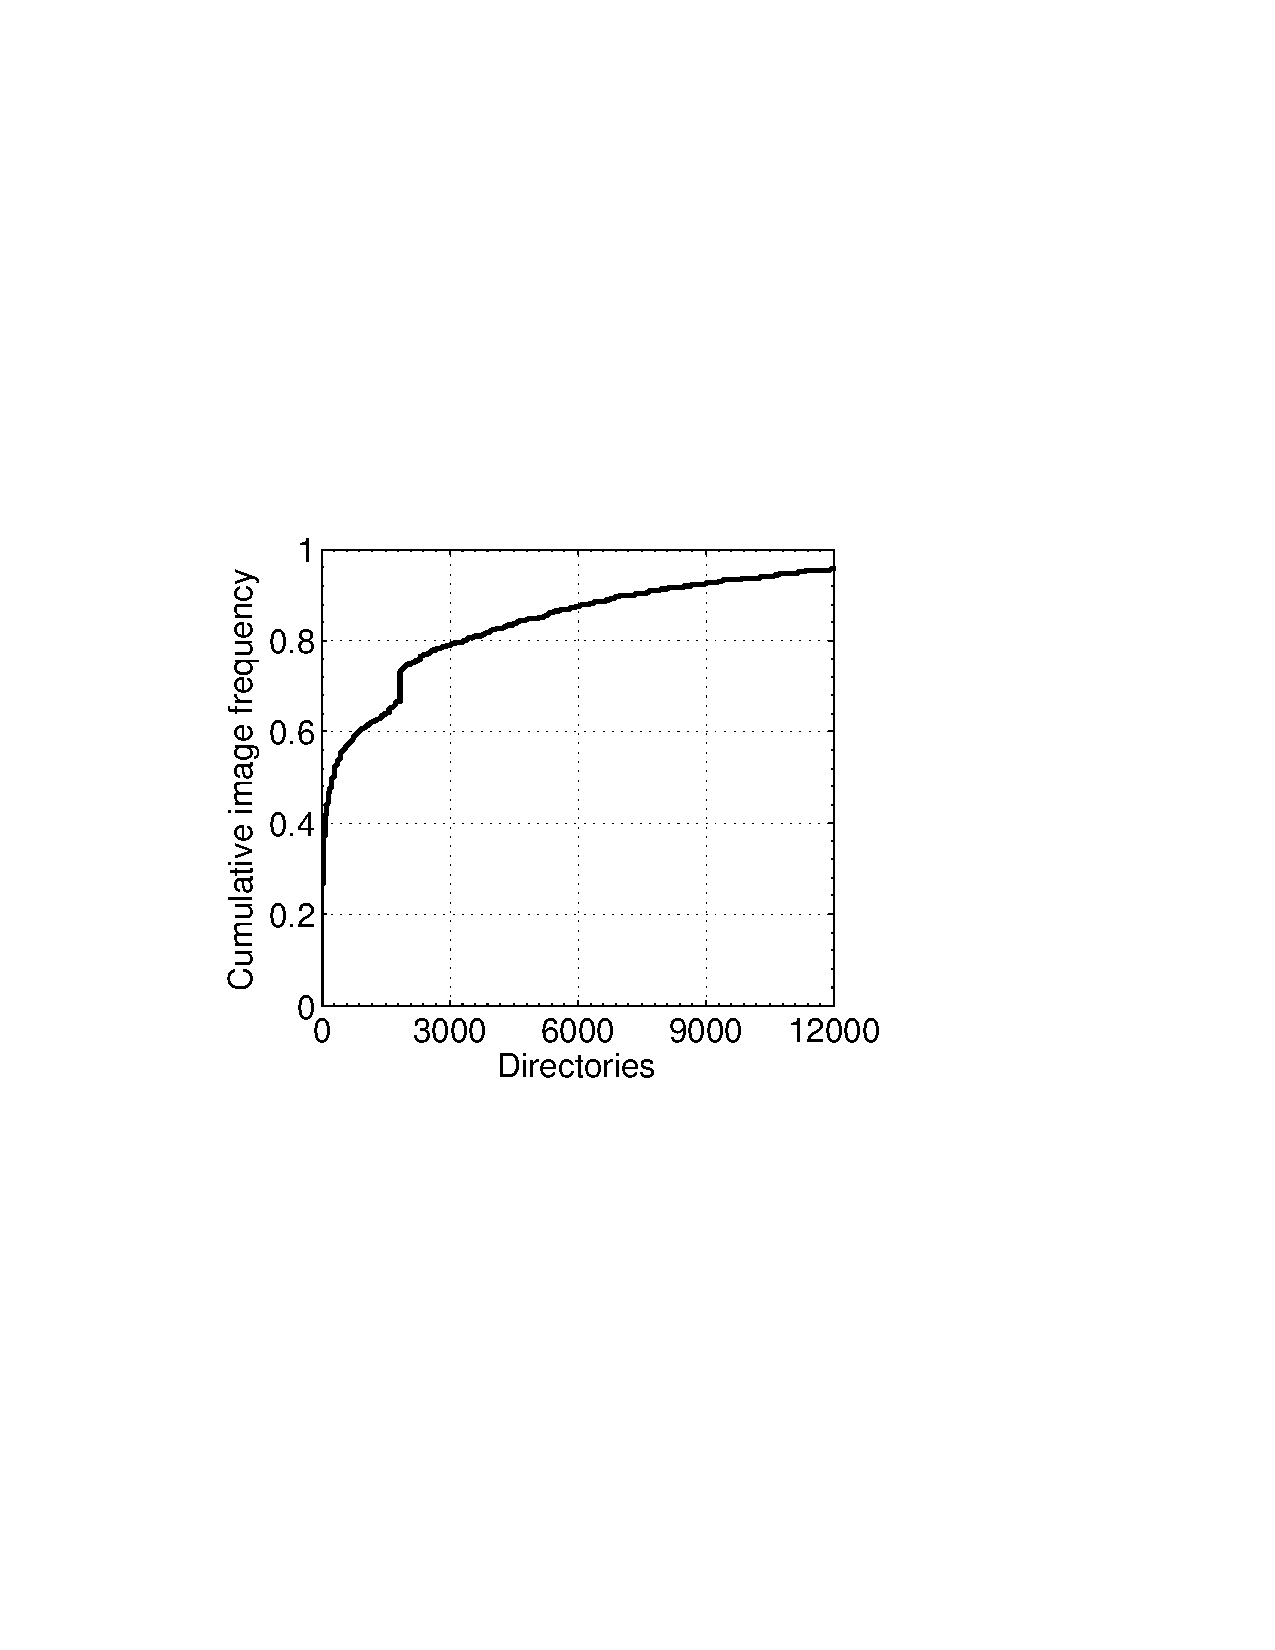
\includegraphics[width=1\textwidth]{graphs/dir.pdf}
%		\caption{CDF of images by\newline directories}
%		\label{fig-dir}
%	\end{minipage}%
%	\begin{minipage}{0.24\textwidth}
%		\centering
%		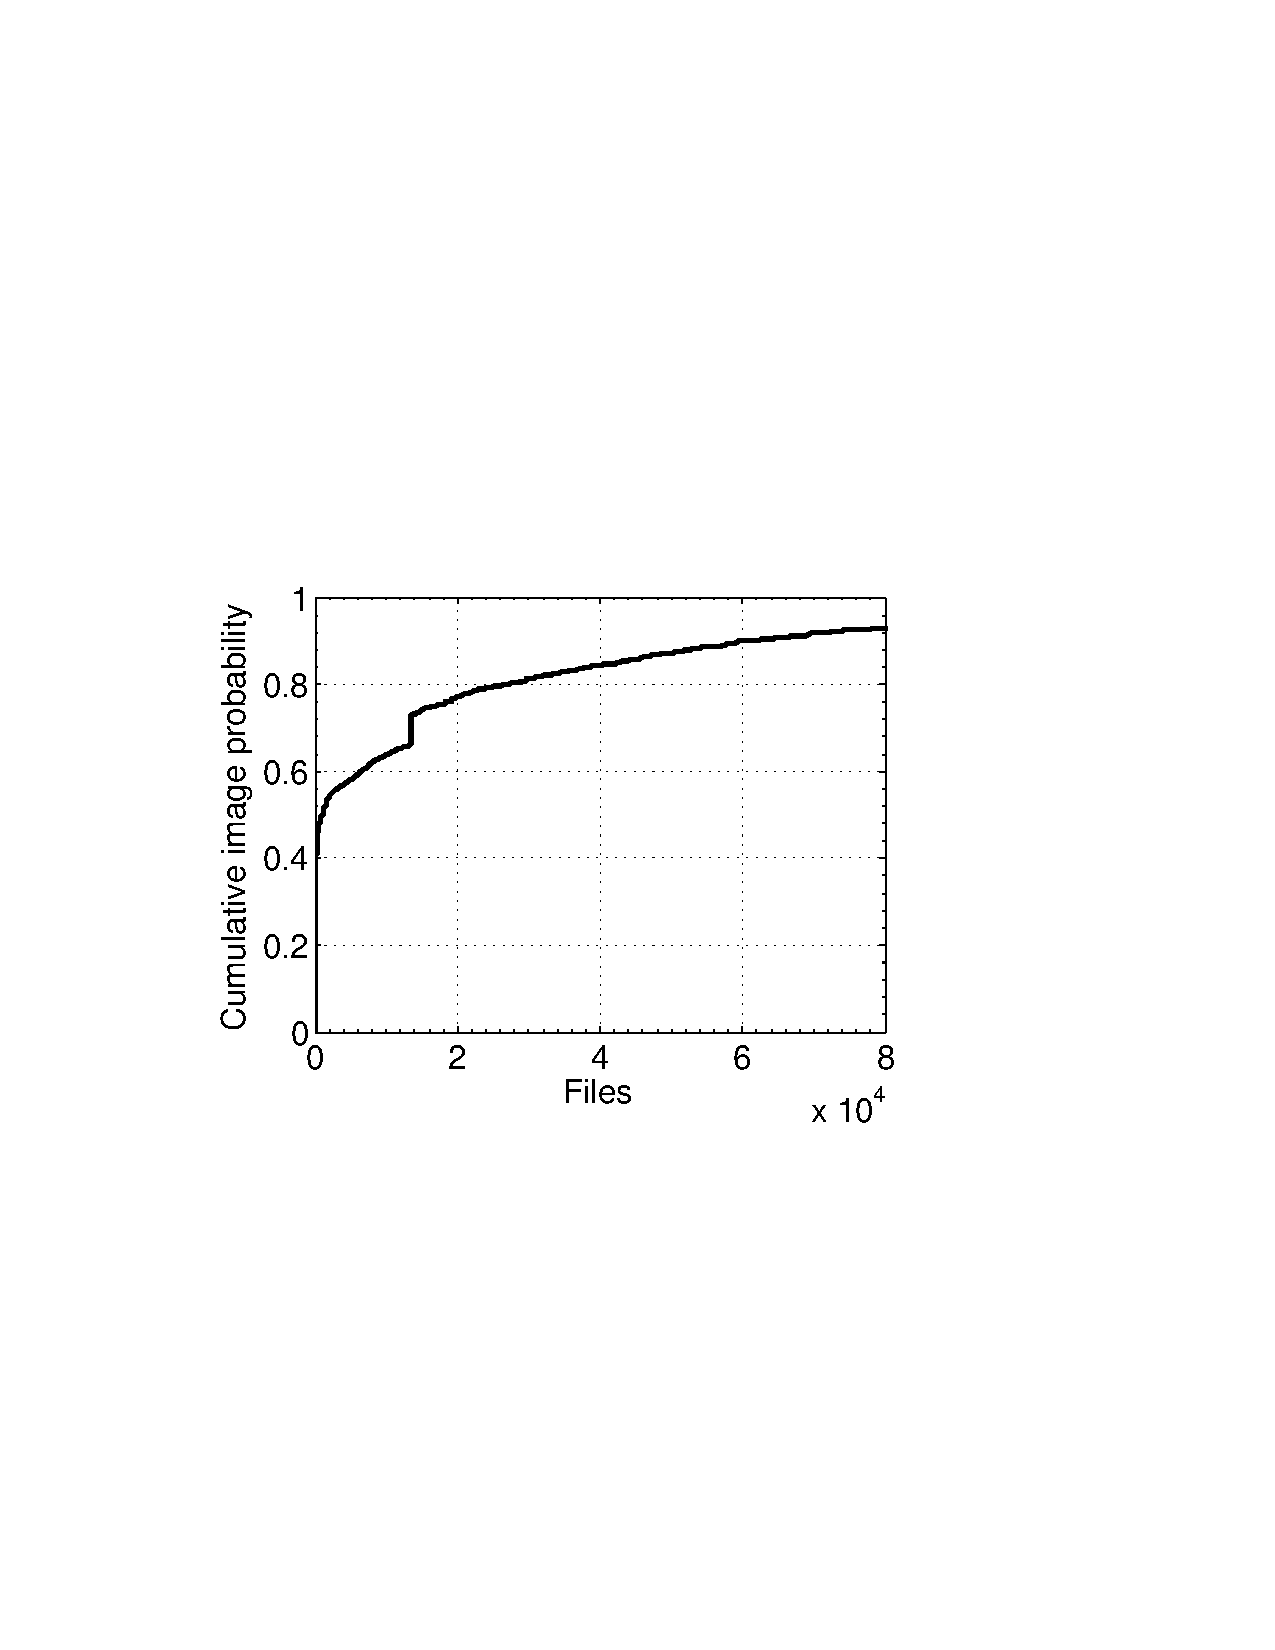
\includegraphics[width=1\textwidth]{graphs/file.pdf}
%		\caption{CDF of images by files}
%		\label{fig-file}
%	\end{minipage}
%\end{figure}

%\begin{figure}[htbp] 
%	\begin{minipage}{0.5\linewidth} 
%		\centering 
%		\includegraphics{circle} 
%		\caption{A Circle} 
%		\label{fig:circle} 
%	\end{minipage}% 
%	\begin{minipage}{0.5\linewidth} 
%		\centering 
%		\includegraphics{rectangle} 
%		\caption{A Rectangle} 
%		\label{fig:rectangle} 
%	\end{minipage} 
%\end{figure}


\subsubsection{User access pattern based preconstruction}

Docker client stores images as lists of layers and layers are shared among different repositories, 
which is similar to Docker registry.
When a client pulls an image from a repository, 
it will first \texttt{pull} the manifest of the image~\cite{docker}~\cite{dockerworkload} and 
parse the manifest to get the layer digests,
then lookup each layer digest against a \emph{local layer index}.
After that it only pulls the layers that have \emph{not been stored locally}.
Theoretically, clients only pull layer once. 
However, some clients may delete several local images and \emph{repull} layers for these images.
%Moreover, kubernetes allows users always \emph{repull} layers no matter these layers locally available or not~\cite{docker}.  
Here, a \emph{repull layer} means same user pull this layer multiple times,
and a \emph{non-repull layer} means users only pull this layer once.

\preconstructcachename~starts parallel slice restoring for layers 
when a \texttt{pull manifest} request is received, 
which is called layer preconstruction.
These preconstructed layer slices are temporally stored in the cache for later \texttt{pull slice} requests.
In this case, slice restoring process and its overhead can be avoided if the requested slice is found in the cache.
Next, we analyze user access patterns to identify which layers in the repository will be pulled by users after 
\texttt{pull manifest} requests.

\paragraph{User access patterns}
Figure~\ref{fig:layer-repull-cdf} shows the CDF of layer repull count.
We see that majority of users don't \emph{repull} layers frequently.
For \texttt{Syd}, only 4\% of layers are repulled by the same clients.
\texttt{Dev} has the highest repull layer ratio of 36\% while 83\% of the repull layers are only repulled twice.
Majority of repulled layers are repulled infrequently.
For example, only 3\% of layers from \texttt{Syd} are repulled more than twice.
Layer from \texttt{Prestage} and \texttt{Lon} have the highest repull frequency.
5\% of layers are pulled more than 6 times.
We also observe that few clients \emph{repull} layers continuously.
The highest layer repull count is 19,300 from \texttt{Lon}.
We think these clients probably deploy containers on a shared platform such as Cloud,
and run ephemeral jobs such as stateless microservices. 
Once the applications are finished, the container images are automatically deleted.
So when users launch containers again, they will repull layers again.

When different clients \texttt{pull} the same repository, 
they will fetch different amount of layers from the repository based on the availability of their local layer dataset.
Even the same clients \texttt{pull} the same repository at different times, 
they will fetch different amount of layers from the repository because their local layer dataset changes over time.
Therefore, a \texttt{pull manifest} requests doesn't usually result in repulling the layers in the repository. 
Here, we define \emph{repulling repository} as 
repulling the layers in the repository for the same client.
Figure~\ref{fig:repo-repull-cdf} shows the CDF of the probability of repository repulling.
The probability of repository repulling is calculated 
as the number of \texttt{pull manifest} resulting in repository repulling divided by 
the total number of \texttt{pull manifest} requests issued by the same client for the same repository.
We see that majority of repositories aren't repulled.
The repull repository ratio ranges from 15\% for \texttt{Prestage} to 43\% for \texttt{Prestage}.
Majority of repull repositories have a low repulling probability.
Only 20\% of repositories from  \texttt{Prestage}, \texttt{Stage}, and 
\texttt{Syd} have a repulling probability higher than 0.5.
And only 20\% of repositories from the rest 4 workloads have a repulling probability higher than 0.33.
We also observe that few repositories' repulling probability are 1, meaning 
every time clients pull these repositories, they always repull the layers in these repositories. 
 
Figure~\ref{fig:client-repull-cdf} shows the client repulling probability.
Client repulling probability is calculated as the number of \emph{repull} layer requests divided by
the number of \texttt{pull} layer requests issued by the same client.
We see that majority of clients do repull layers but the probability is low.
60\% of clients from \texttt{Prestage}, \texttt{Dev}, \texttt{Lon}, and \texttt{Fra} have a repulling probability lower than 0.1.
55\% of clients from both \texttt{Dal} and \texttt{Stage} have a repulling probability lower than 0.1.
Less clients have repulling probability range between 0.1 to 0.7.
10\%-30\% of clients have a repulling probability ranged from 0.2-0.7 across 7 workloads.
We find few clients repull layers continuously.
2\%-12\% of clients have a repulling probability higher than 0.9 from workloads:
\texttt{Dal}, \texttt{Dev}, \texttt{Fra}, \texttt{Prestage},
\texttt{Stage}, \texttt{Syd}, and \texttt{Lon}.

\paragraph{Monitor user access patterns}
To monitor user access patterns,
\preconstructcachename~first uses a RLmap to record repository-layer relationship.
If user~\emph{u} \emph{pushes} a  layer~\emph{l} to a repository~\emph{r},
\preconstructcachename~will add an new entry (\emph{l}) in RLmap denoted as RLmap[\emph{r, l}]. 
%Based on user access patterns,
\preconstructcachename~ also maintains a URLmap for keeping track of user access patterns.
To identify a user, 
we extract \emph{user end host address} (\emph{r.client}) from each request (\emph{r}). 
Each URLmap entry maintains a user profile for each user \emph{u} denoted as URLmap[\emph{u}]. %as shown in Figure~\ref{xxx}.
User profile contains a list of repository profiles for each accessed repository \emph{repo} denoted as URLmap[\emph{u, repo}],
and each repo profile contains a list of layer profiles for each accessed layer \emph{l}  denoted as URLmap[\emph{u, repo, l}].
Note that layer profiles can be shared among different repo profiles for the same user.
If user~\emph{u} \texttt{pull}s a layer~\emph{l} from a repository~\emph{repo},
\preconstructcachename will update layer profile URLmap[\emph{u, repo, l}] with the corresponding layer repull count, and calculate
repository repulling probability and user repulling probability for the corresponding repository profile and user profile.
%Each node records the following history information: (\emph{Get\_cnt}, \emph{Put\_cnt}, \emph{last\_access\_time}). a child node layer~\emph{L} to parent node~\emph{R}
%User profile records the user repulling probability $u.rp$ for client $u$.
%If $u.rp$ is greater than threshold $\theta_{crp}$, this user has a high probability of repulling layers.
%Repo profile records repository repulling probability $u.r.rp$ for repository $r$.
%If $u.r.rp$ is greater than threshold $\theta_{rrp}$, this repository is a popular repulling repository for this user.
%Layer profile records layer repull count $u.l.R$ for layer $l$.
%If $u.l.R$ is greater than threshold $\theta_{R}$, this layer is a popular repull layer for this user.

\paragraph{Preconstruction algorithm}
\begin{algorithm}
\scriptsize 
	\caption{Layer preconstruction}
	\label{alg:prefetch}
	\KwIn{\\
		$\theta_{rpc}$: Threshold for repull layers to be preconstructed. \\
		$RLmap$: Repository to layer map. \\
		$ULmap$: User to layer map.  \\
		$LayerRecipes$: Layer recipes. \\
		$SliceRecipes$: Slice recipes.\\
	}
	\emph{r} $\leftarrow$ \texttt{request received}\\
	\uIf{r = GET manifest}
		{
			difference $\gets$ \emph{RLmap[r.repo]} $-$ \emph{ULmap[r.client]} \\
			intersection $\gets$ \emph{RLmap[r.repo]} $\bigcap$ \emph{ULmap[r.client]} \\
			
			targets $\leftarrow$ difference \\
			\ForEach{layer in intersection} 
			{ \If{ layer.rpcnt $>$ $\theta_{rpc}$}{
				targets	$\leftarrow$ layer
				}
			}
			\ForEach{layer in targets} {
				master $\leftarrow$ \emph{LayerRecipes[layer].master} \\
				\texttt{Notify} master `PRECONSTRUCT layer' \\
			}
		}
	
		\uElseIf{r = PRECONSTRUCT layer}
		{
			\If{r.layer not in DiskCache}{
				workers $\leftarrow$ \emph{LayerRecipes[r.layer].workers} \\
				\ForEach{worker in workers} {
					%{\scriptsize $/*$\textit{sliceid = r.layer+worker}}\\ 
					slices $\leftarrow$ \texttt{GET slice from} worker `GET slice' \\
				}
				layer $\leftarrow$ \texttt{Concatenate} slices \\
				
				DiskCache $\gets$ layer \\
				{\tiny{$/*$\texttt{Set timer for layer}} $/*$}\\
			}
		}
	
		\uElseIf{r = GET slice}
		{
			slice $\leftarrow$ \texttt{Construct by following} \emph{SliceRecipes[r.slice]} \\
			
			\texttt{Serve} slice \\
		}
	
%		\uElseIf{r = PUT layer}
%		{
%				\emph{LayerCache} $\leftarrow$ \texttt{cache} \emph{r.layer} \\
%				\texttt{update} \emph{RLmap[r.repo, r.layer]} \\
%		}
%		\uElseIf{r = GET layer} 
%		{
%			{\tiny\texttt{/* r.layer has not been deduplicated   /}} \\
%				\eIf{r.layer in cache}
%				{
%					\emph{cache hit for layer} \\
%					\texttt{Serve} layer \\
%				} 
%				{
%					workers $\leftarrow$ \emph{LayerRecipes[layer].workers} \\
%					\ForEach{slave in slaves} {
%						slices $\leftarrow$ \texttt{GET} worker `GET layer'slice' \\
%					}
%					layer $\leftarrow$ \texttt{Concatenate} slices \\
%					\texttt{Serve} layer
%					LayerCache $\gets$ layer \\
%				}
%		}
%		\texttt{update} \emph{ULmap[r.client, r.repo, r.layer]} \\
		
\end{algorithm}




Algorithm~\ref{alg:prefetch} shows when to preconstruct slices for a layer
based on observed user access pattern.
When a \texttt{GET manifest} request \emph{r} is received,
\preconstructcachename~lookups the requested repository \emph{r.repo}'s layers from RLmap
and get a list of corresponding layers.
After that, it compares against the layers lookuped from URLmap[\emph{r}] (denoted as URLmap[\emph{r}].layers)
and gets two groups of layers: \emph{newLayers} and \emph{oldLayers}.
\emph{newLayers} means the layers that belongs to \emph{r.repo} but haven't been pulled by client \emph{r.client}.
While \emph{oldLayers} means the layers that belongs to both of them.
\preconstructcachename~will first restore the slices for \emph{newLayers} because 
they are not locally available to \emph{r.client}.    
For \emph{oldLayers}, 
if an \emph{oldLayer} has a higher repull count and \emph{r.repo} as well as \emph{r.client} have a higher repulling probability,
then \preconstructcachename~will restore its slices and cache them.
If a \emph{PUT} layer request is received, RLmap and URLmap will be updated accordingly.

If a \emph{GET} layer request is received, it means that \emph{r.layer} has not been deduplicated.
\preconstructcachename~will cache \emph{r.layer} if cache miss happens on \emph{GET} layer request as shown in Algorithm~\ref{alg:prefetch}.
If a \emph{GET} slice request is received, meaning that \emph{r.layer} has already been deduplicated into deduplicated slices,
\preconstructcachename~will check if the requested \emph{r.slice} exists in the cache.
If not,
\dedupname system~will start restoring \emph{r.slice} and also put it in cache.
In the end, \preconstructcachename~will update URLmap with corresponding repull count and repull probability.

\subsubsection{User access pattern  based cache replacement}
%\begin{figure*}[t]
%		\begin{minipage}{0.32\linewidth}
%			\centering
%			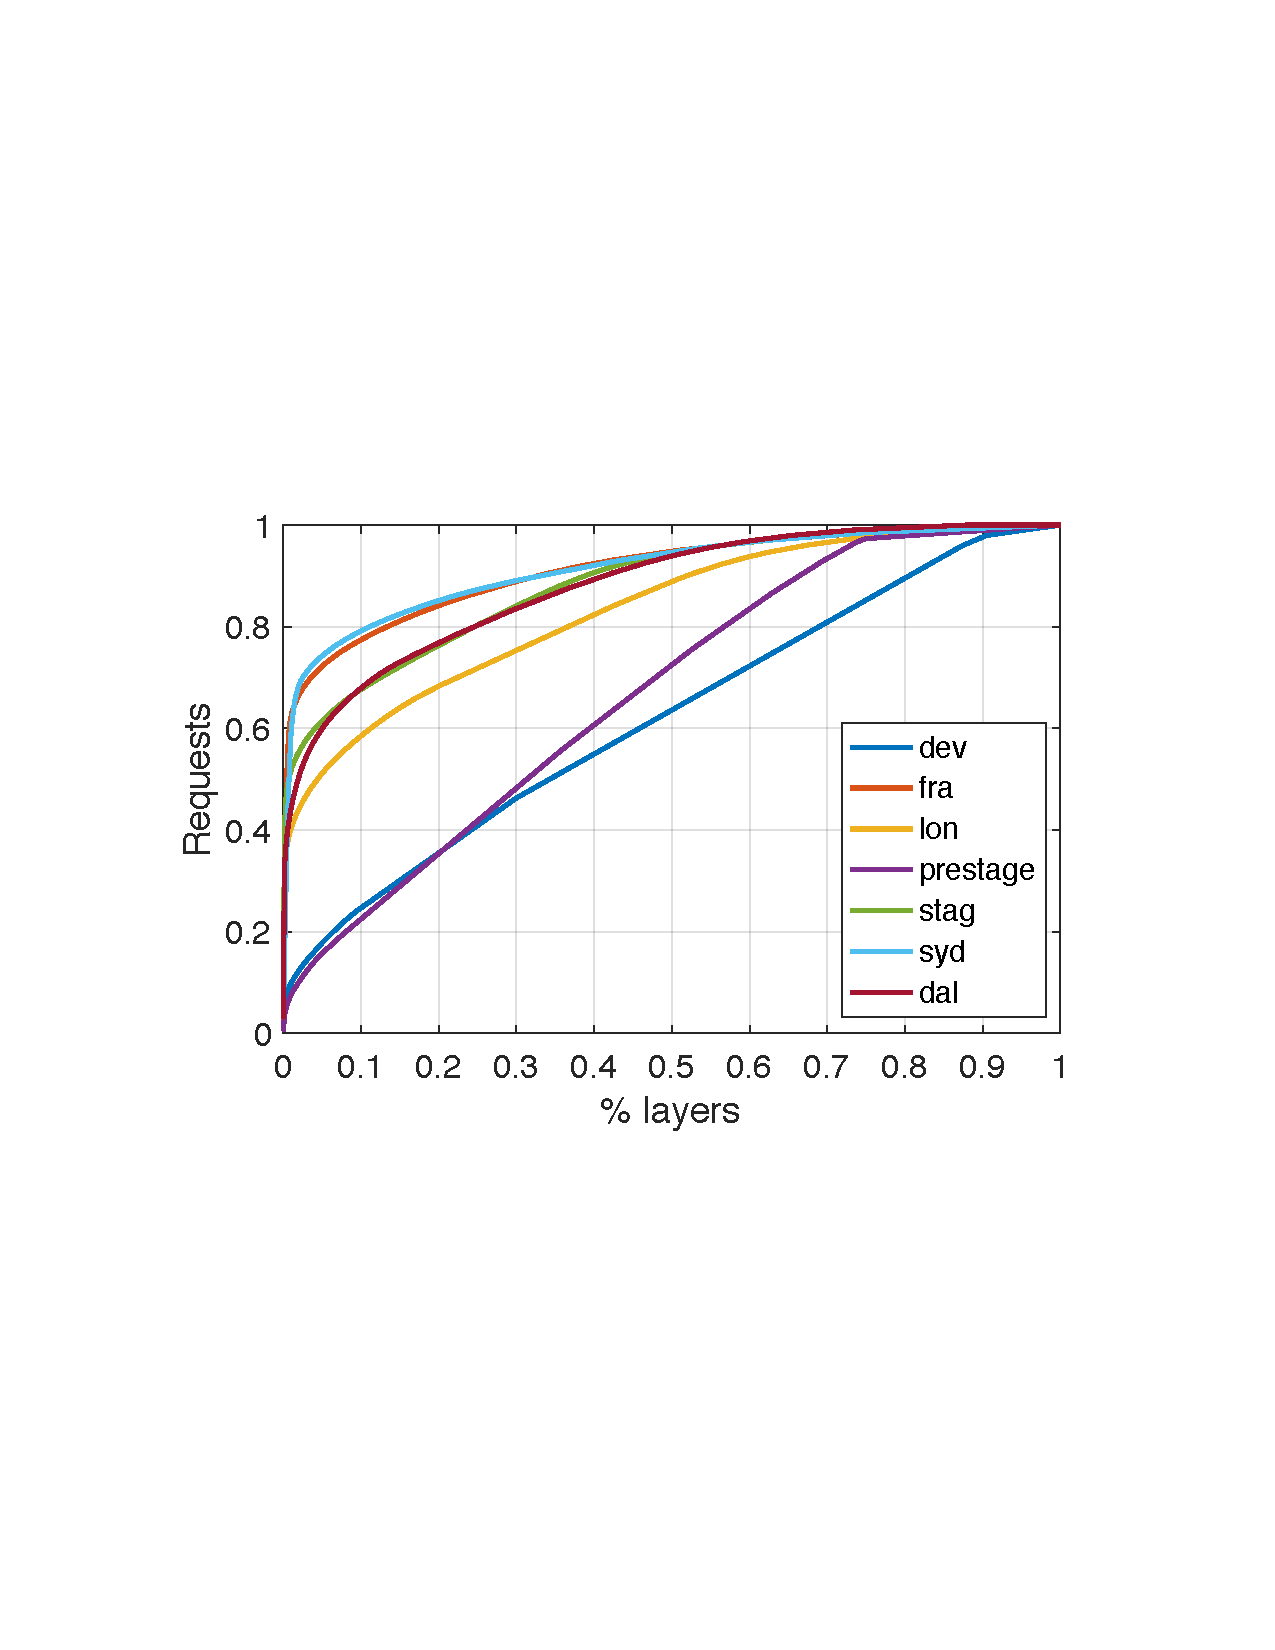
\includegraphics[width=1\textwidth]{graphs/layer_skewness.pdf}
%			%\caption{CDF of layer  count.}
%		%	\vspace{-3pt}
%			\label{fig:layer-skenwess}
%		\end{minipage}
%			\begin{minipage}{0.32\linewidth}
%				\centering
%				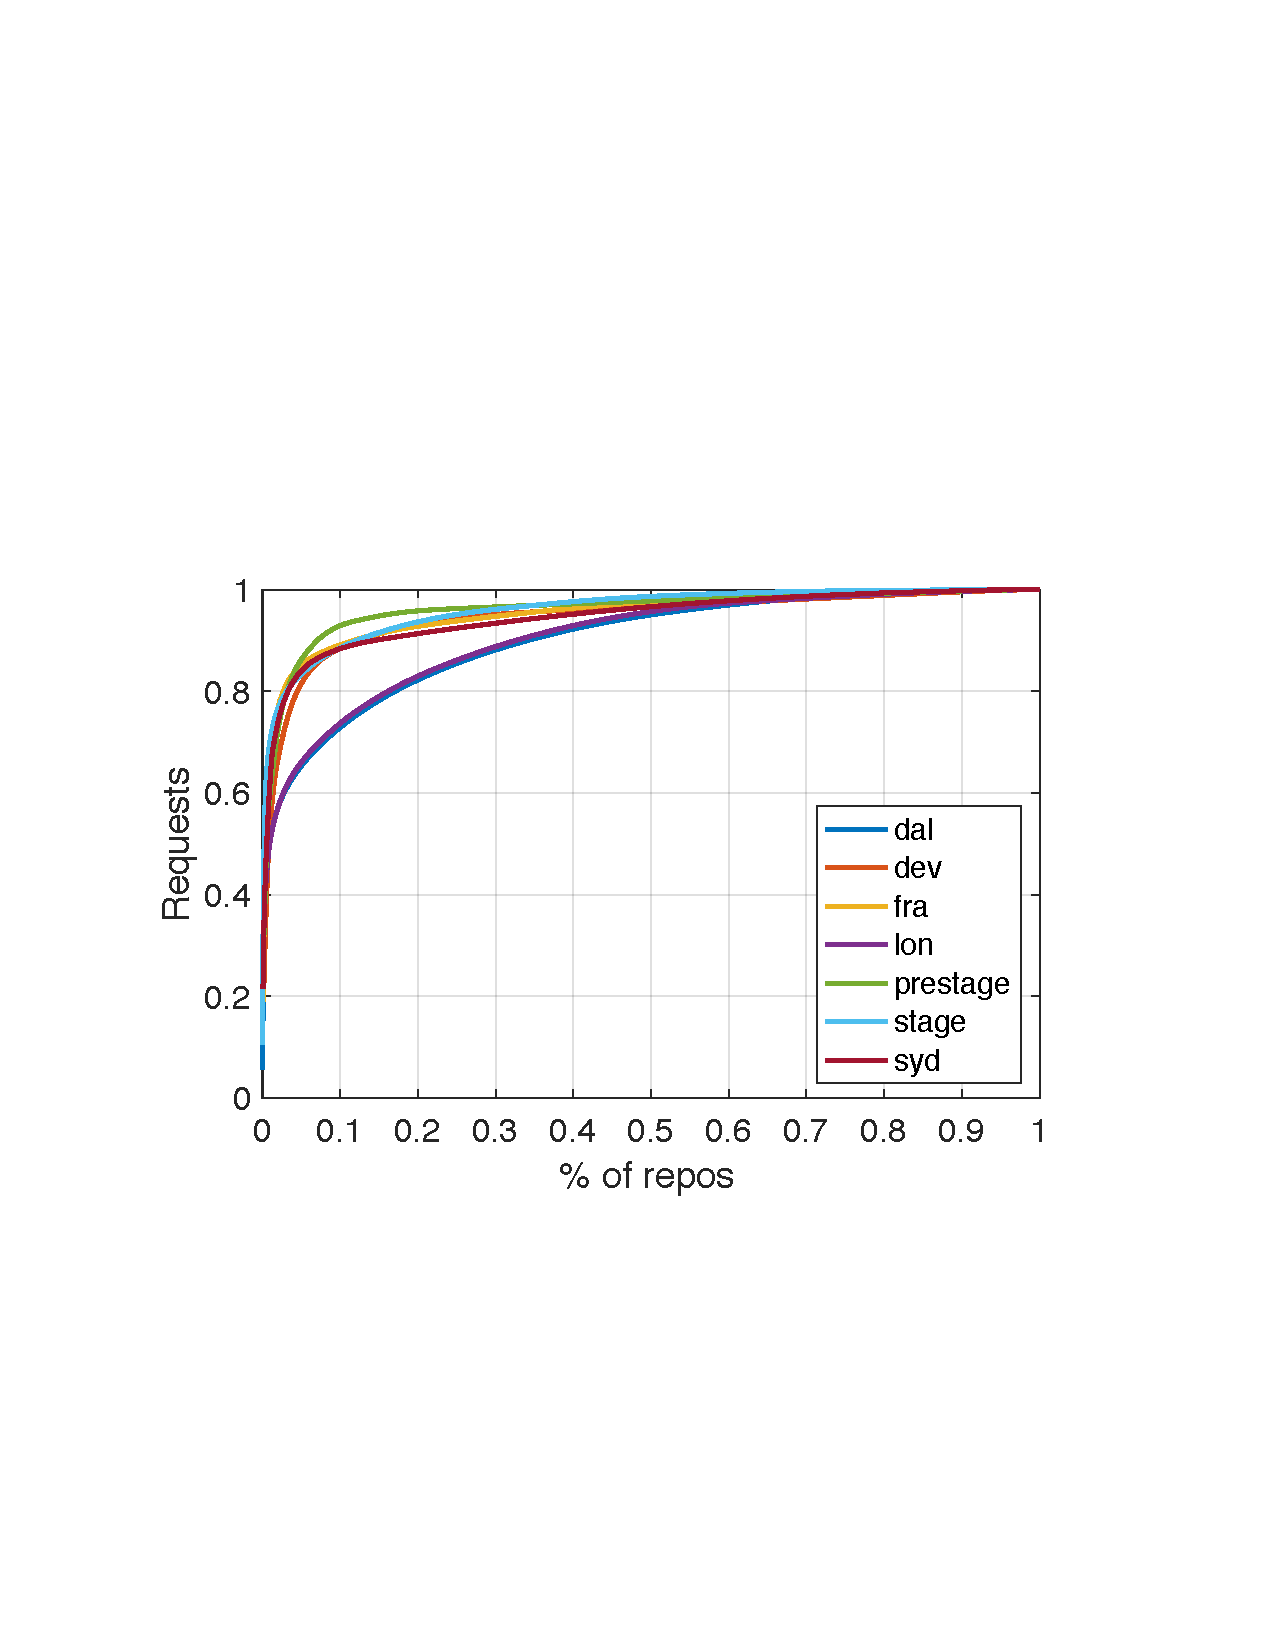
\includegraphics[width=1\textwidth]{graphs/repo-skewness.pdf}
%				%\caption{PDF of repository repulling probability.}
%				%	\vspace{-3pt}
%				\label{fig:repo-skewness}
%			\end{minipage}
%		\hfill
%		\begin{minipage}{0.32\linewidth}
%			\centering
%			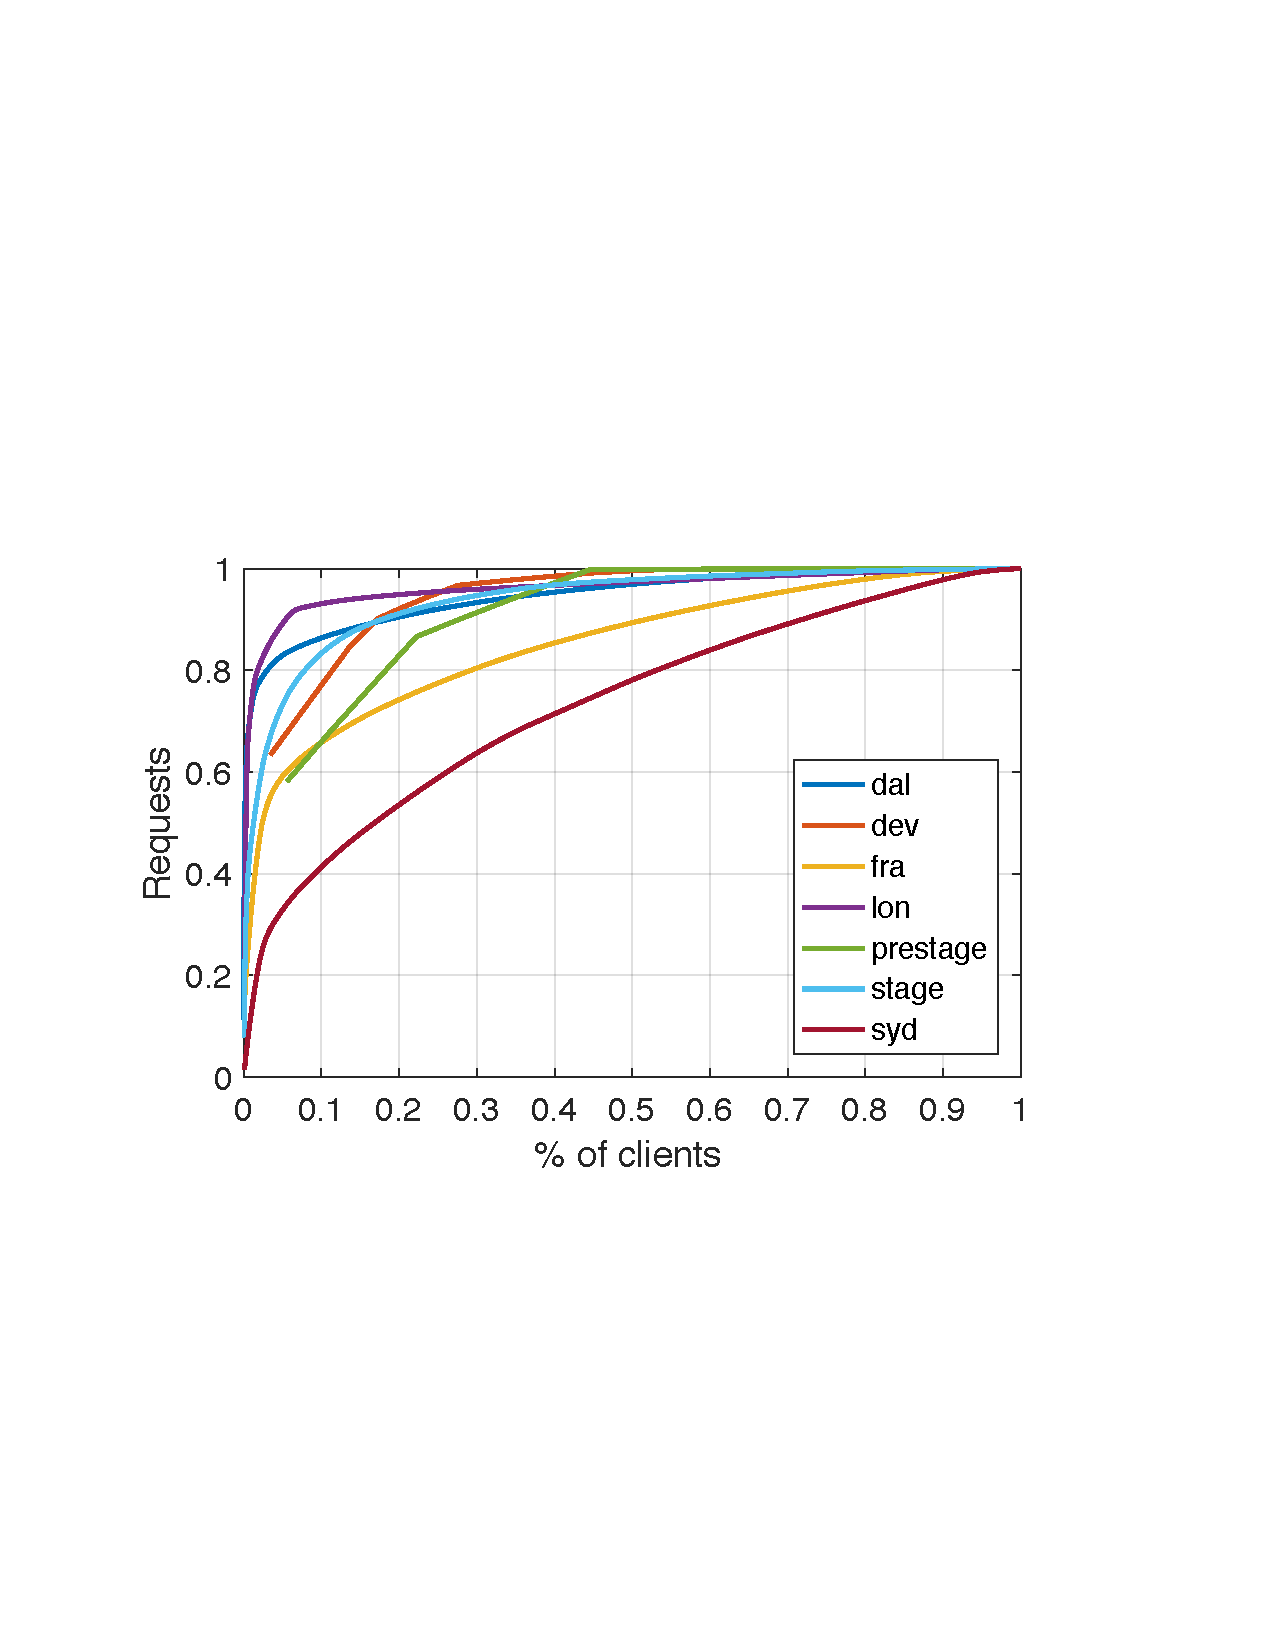
\includegraphics[width=1\textwidth]{graphs/client-skewness.pdf}
%			%\caption{PDF of client repulling probability.}
%			%	\vspace{-3pt}
%			\label{fig:client-skewness}
%			
%		\end{minipage}
%\caption{PDF of probability for layers, repositories, and clients.}
%%	\label{}
%\end{figure*}

\begin{figure*}[!t]
	\centering
	\subfigure[Layer repull count]{
		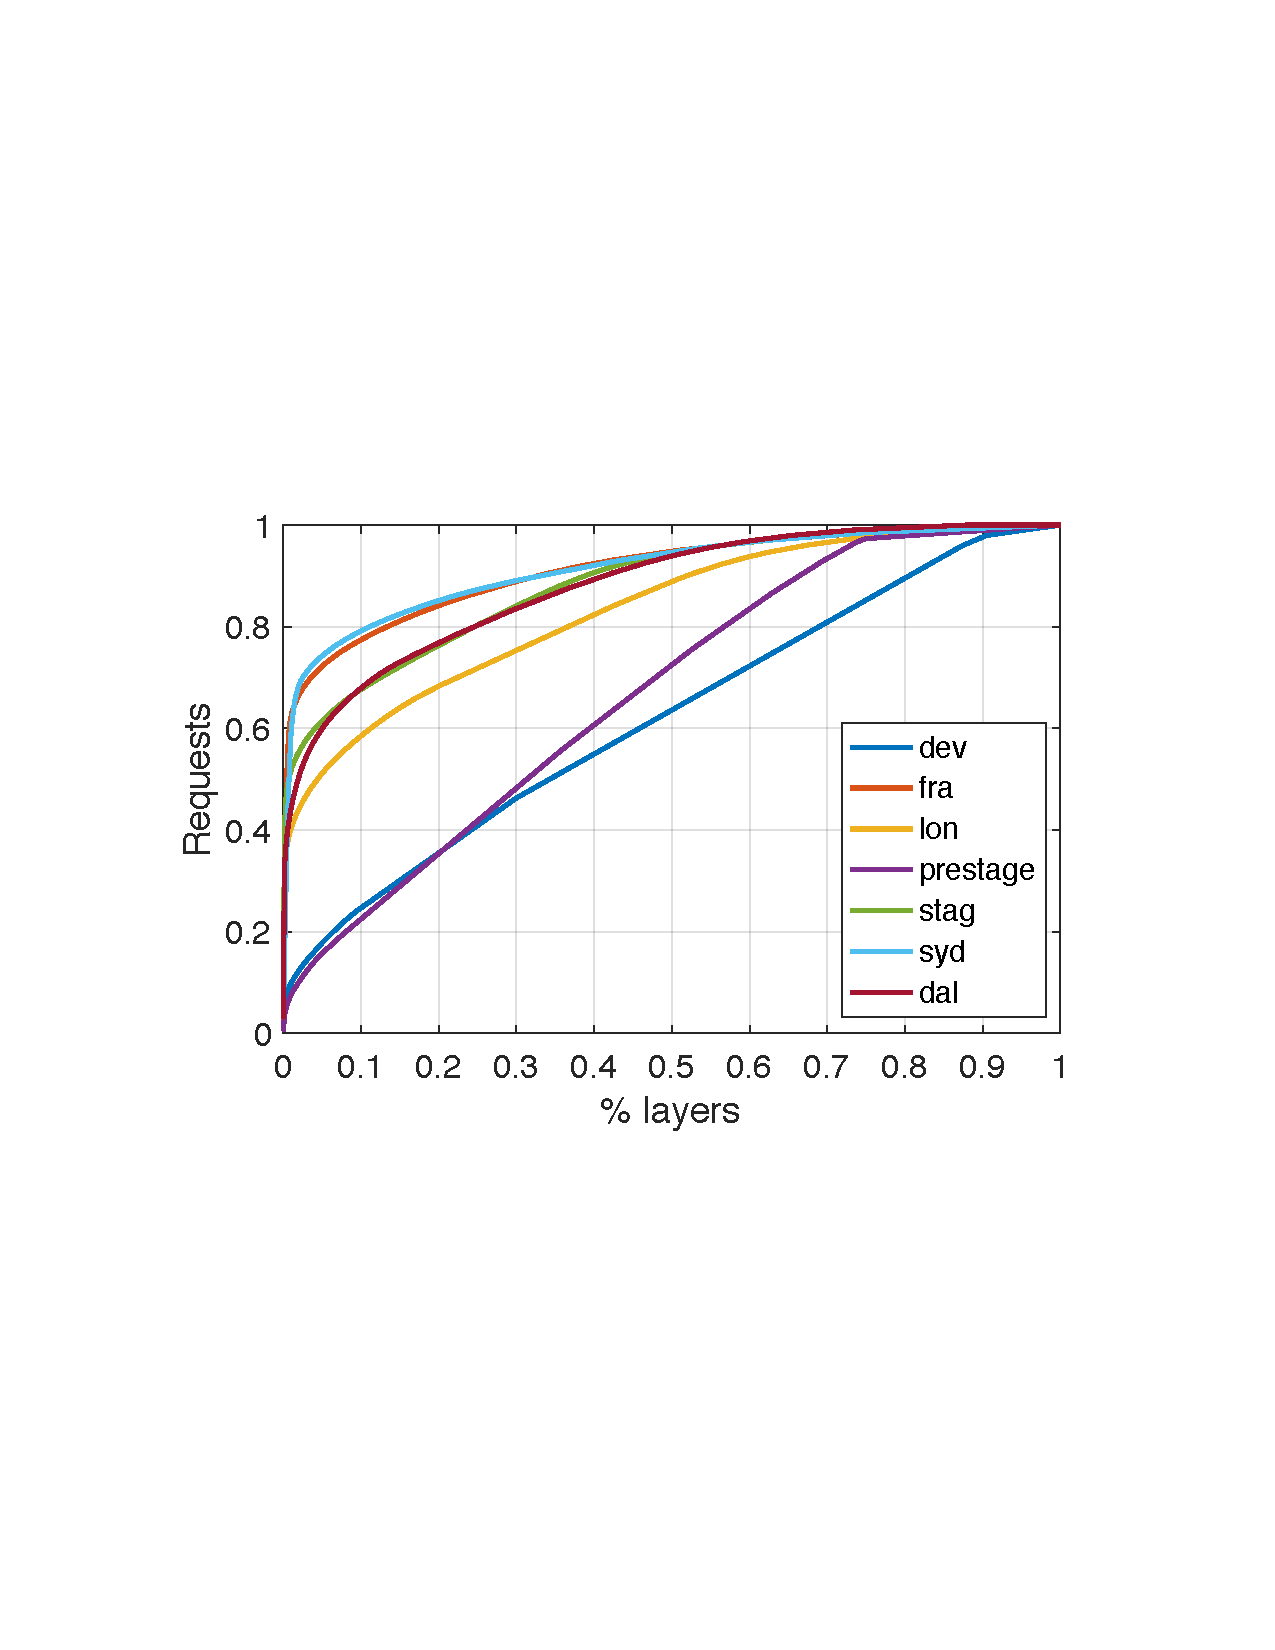
\includegraphics[width=0.2\linewidth]{graphs/layer_skewness.pdf}
		\label{fig:layer-skenwess}
	}
	\subfigure[Repository repulling probability]{
		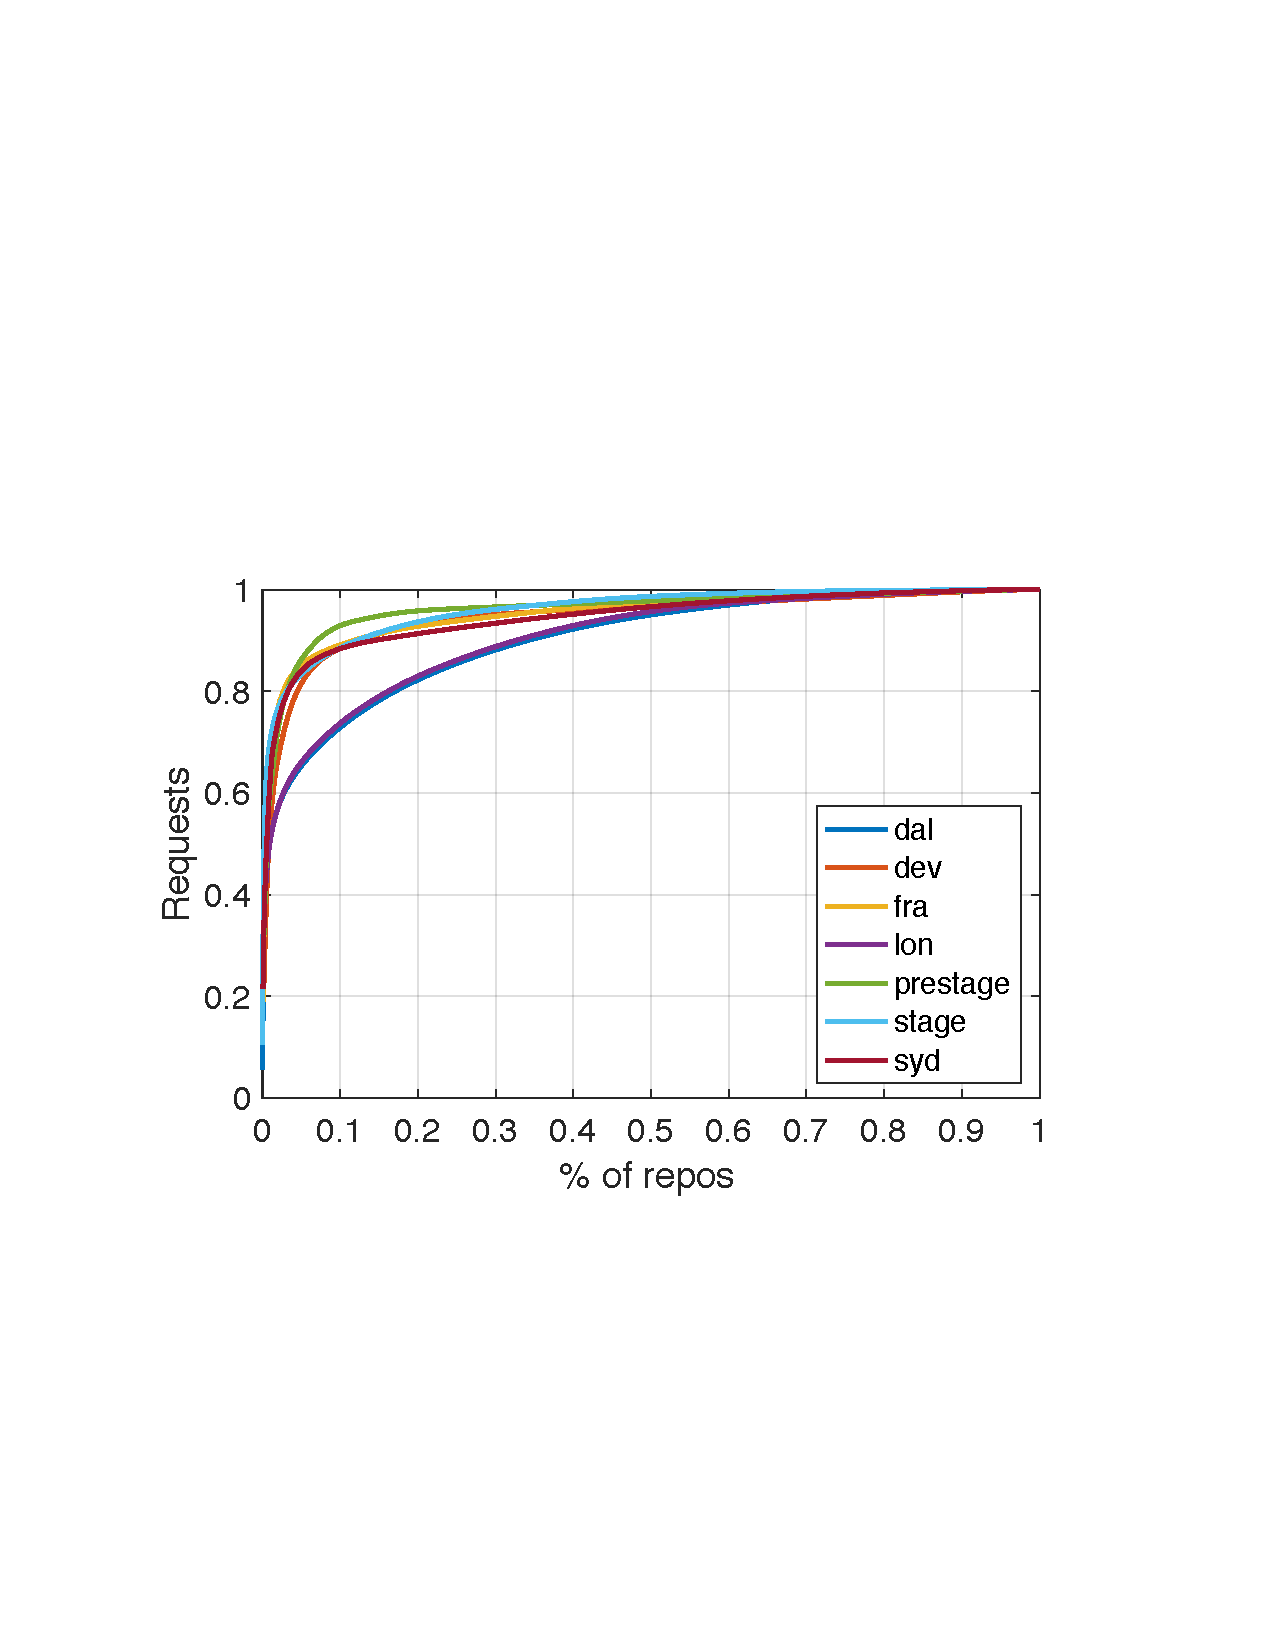
\includegraphics[width=0.2\linewidth]{graphs/repo-skewness.pdf}
		\label{fig:repo-skewness}
	}
	\subfigure[Client repulling probability]{
		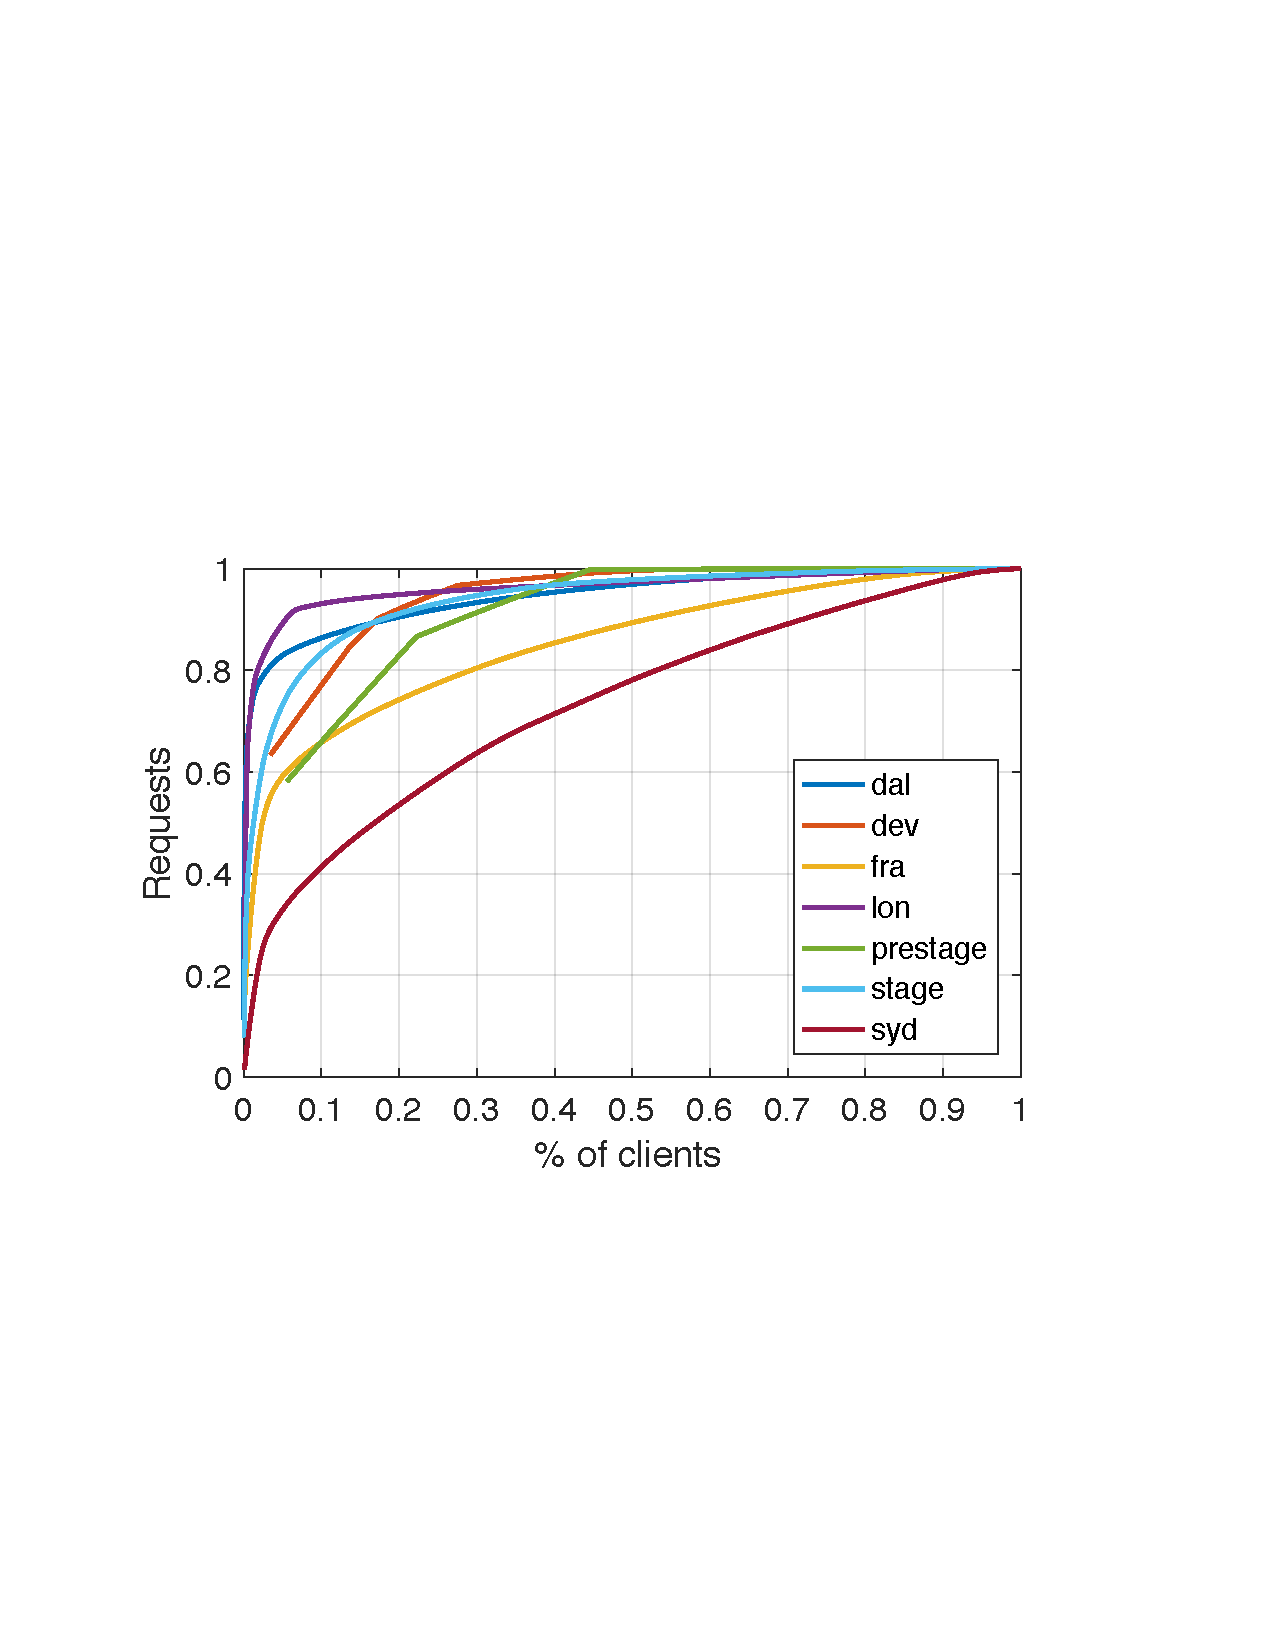
\includegraphics[width=0.2\linewidth]{graphs/client-skewness.pdf}
 	\label{fig:client-skewness}
	}
\caption{PDF of probability for layers, repositories, and clients.}
	\label{fig-skewness}
\end{figure*}
%\begin{figure*}[t]
%		\begin{minipage}{0.32\linewidth}
%			\centering
%			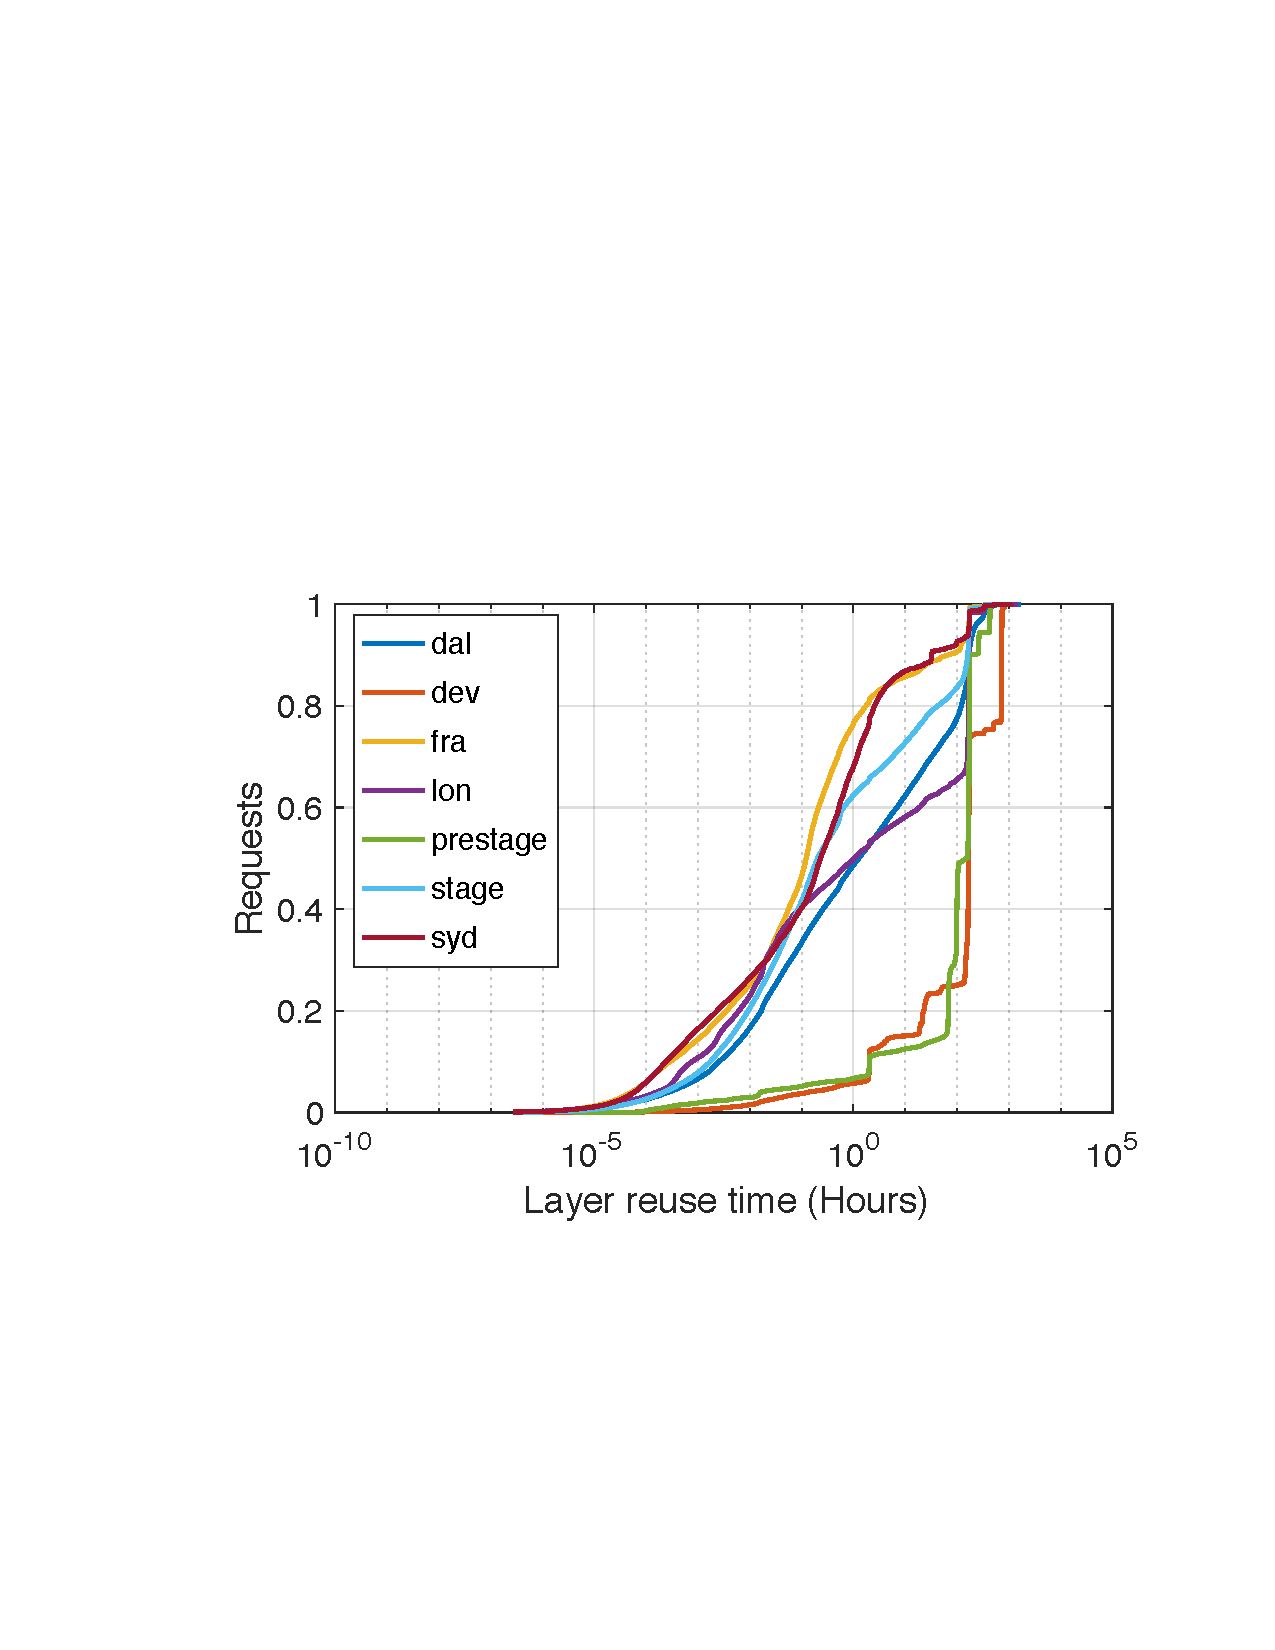
\includegraphics[width=1\textwidth]{graphs/layer-reusetime.pdf}
%		%	\caption{CDF of layer reuse time.}
%		%	\vspace{-3pt}
%			\label{fig:layer-reuse}
%		\end{minipage}
%			\begin{minipage}{0.32\linewidth}
%				\centering
%				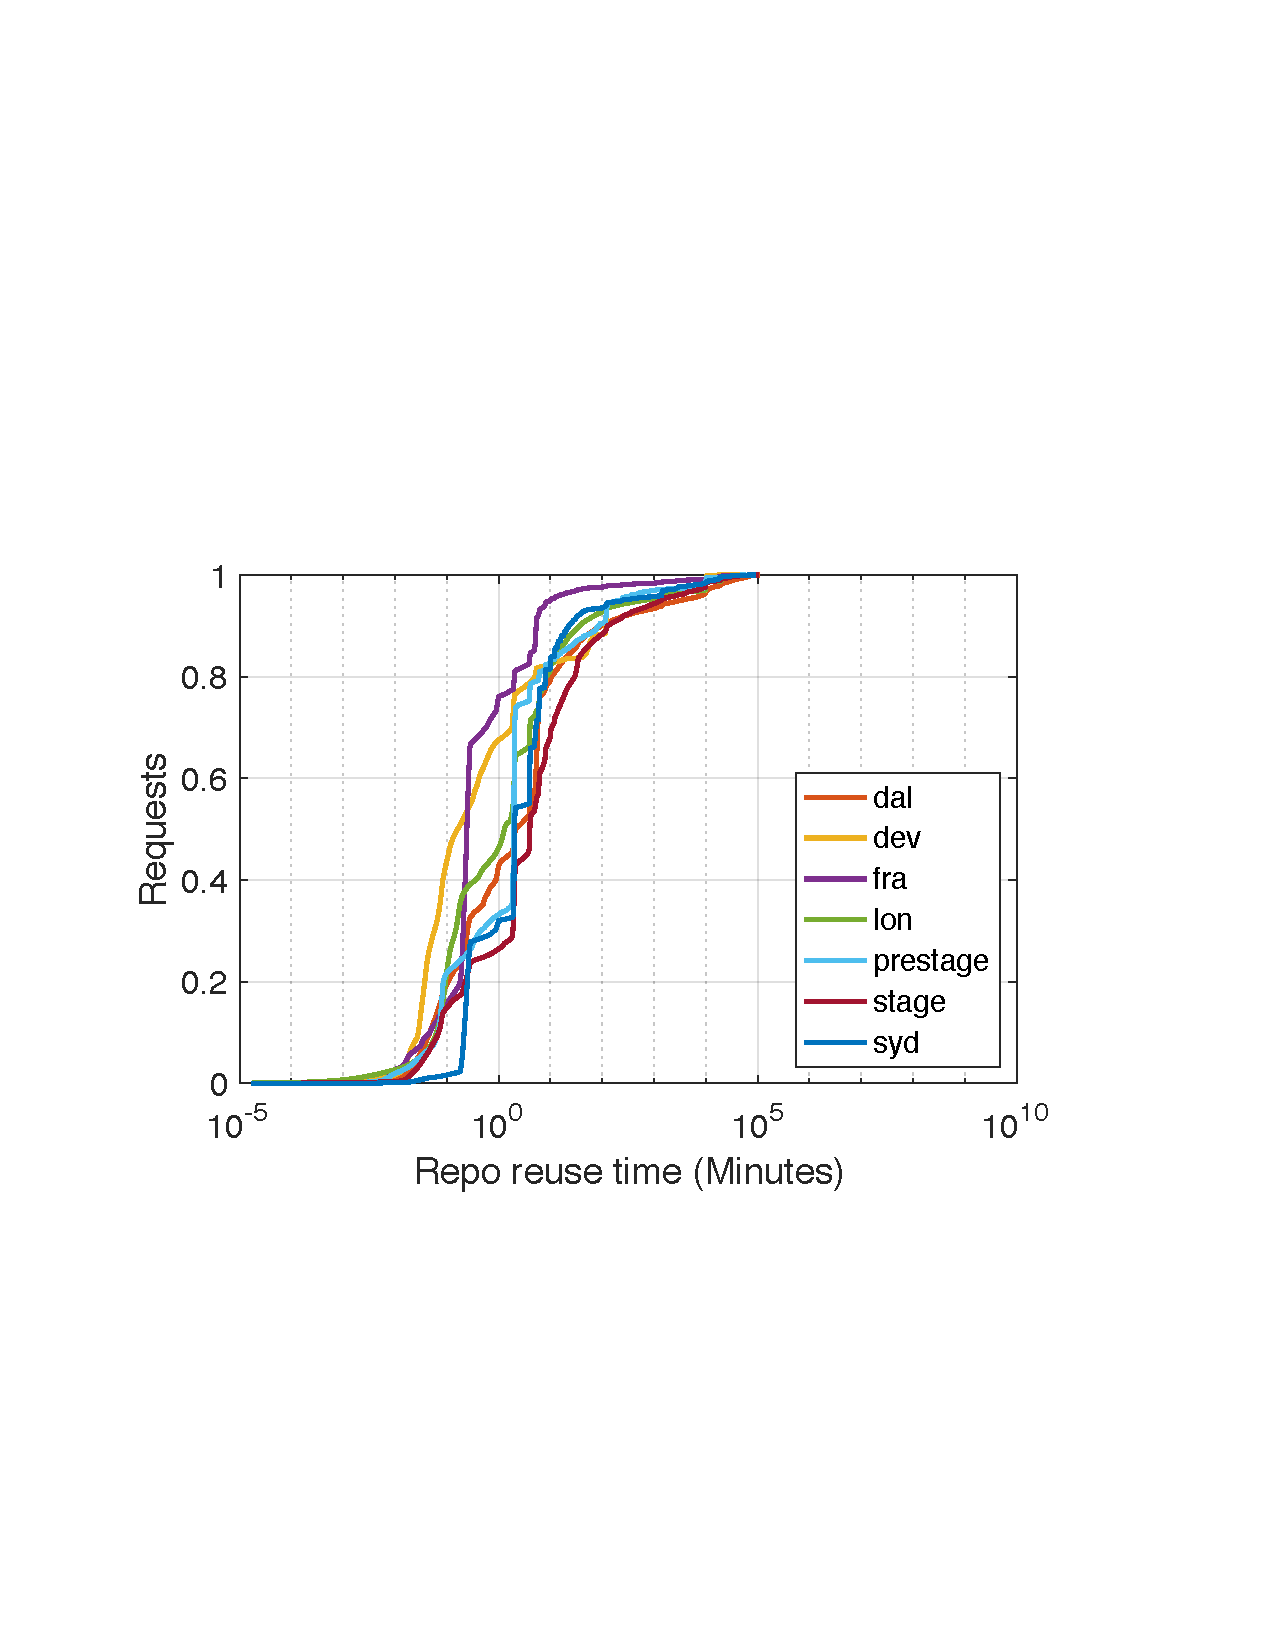
\includegraphics[width=1\textwidth]{graphs/repo-reusetime.pdf}
%			%	\caption{PDF of repository reuse time.}
%				%	\vspace{-3pt}
%				\label{fig:repo-reuse}
%			\end{minipage}
%		\begin{minipage}{0.32\linewidth}
%			\centering
%			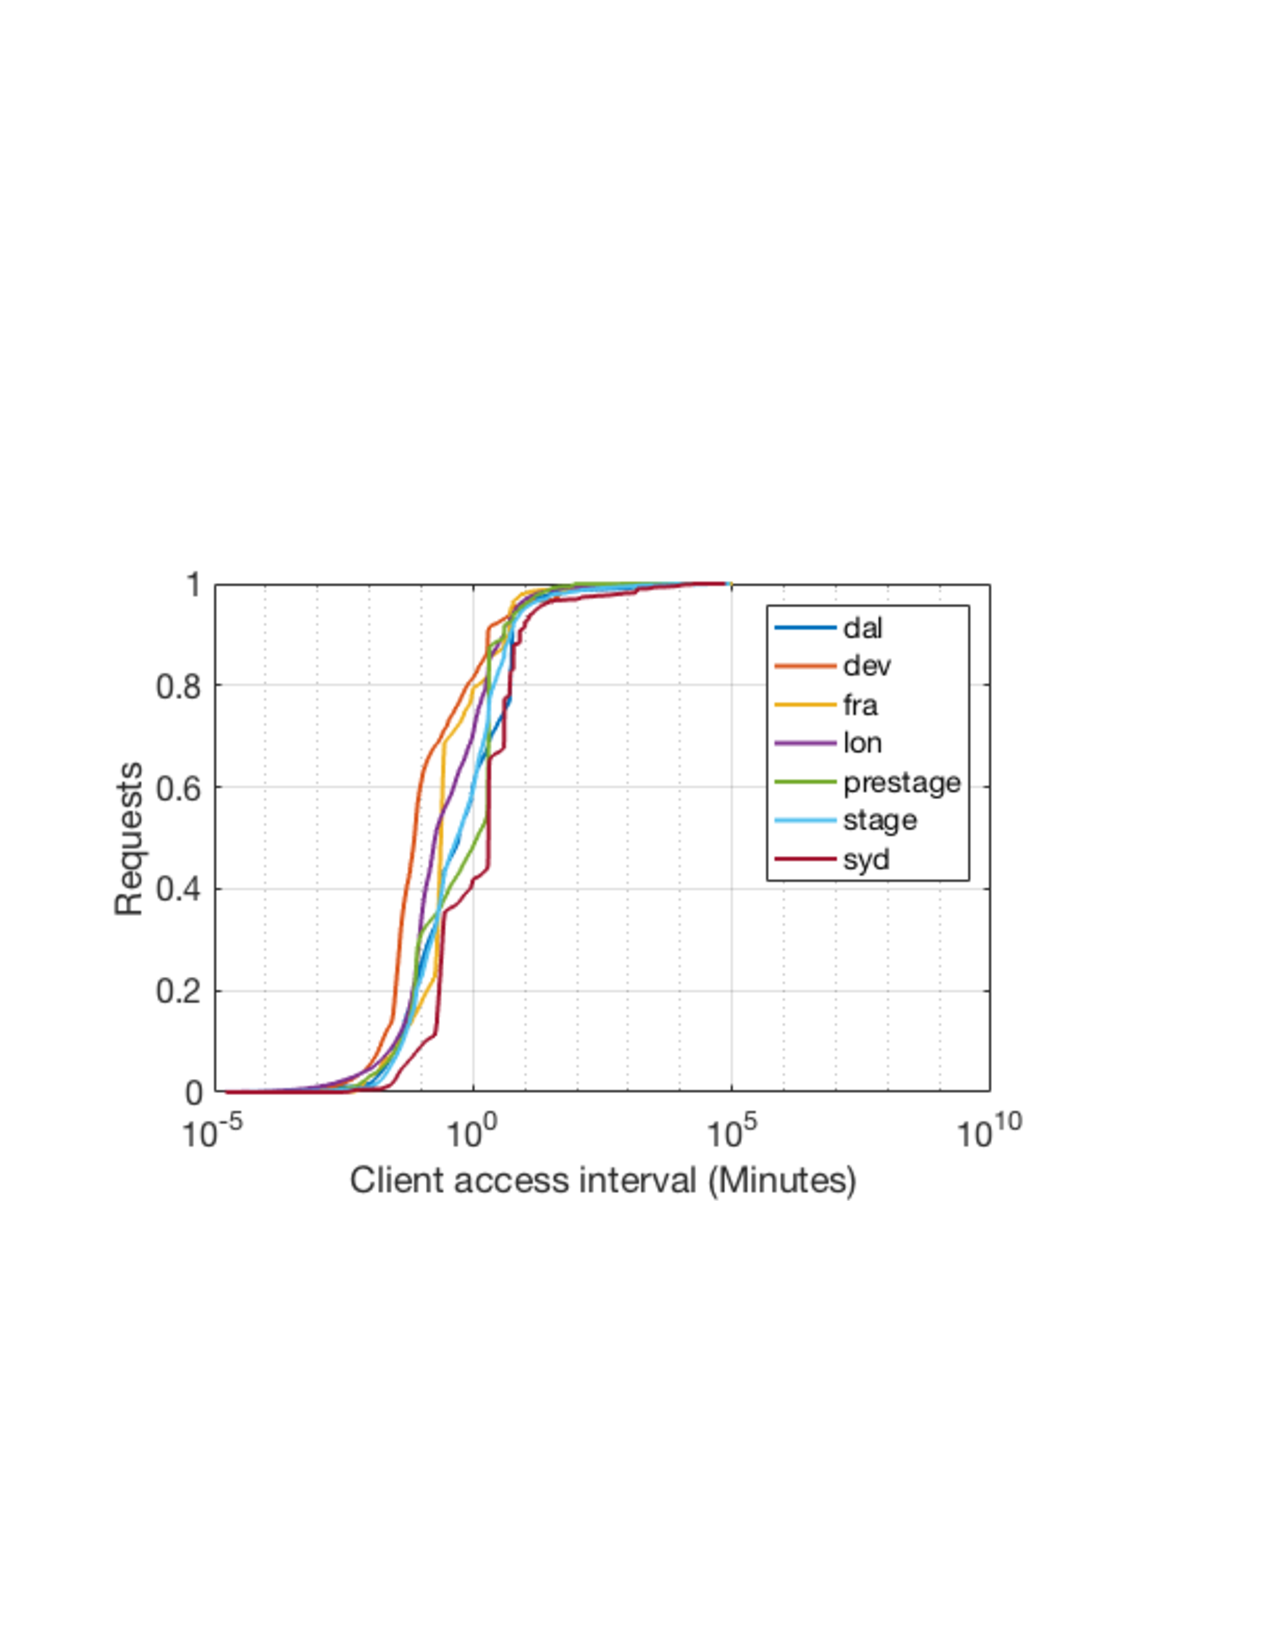
\includegraphics[width=1\textwidth]{graphs/user-intervals.pdf}
%			%\caption{PDF of client access intervals.}
%			%	\vspace{-3pt}
%			\label{fig:user-interval}
%		\end{minipage}
%	\caption{CDF of reusetime for layers, repositories and clients' access intervals.}
%	\label{fig:layer-reuse}
%\end{figure*}
\begin{figure}[t]
	\centering
	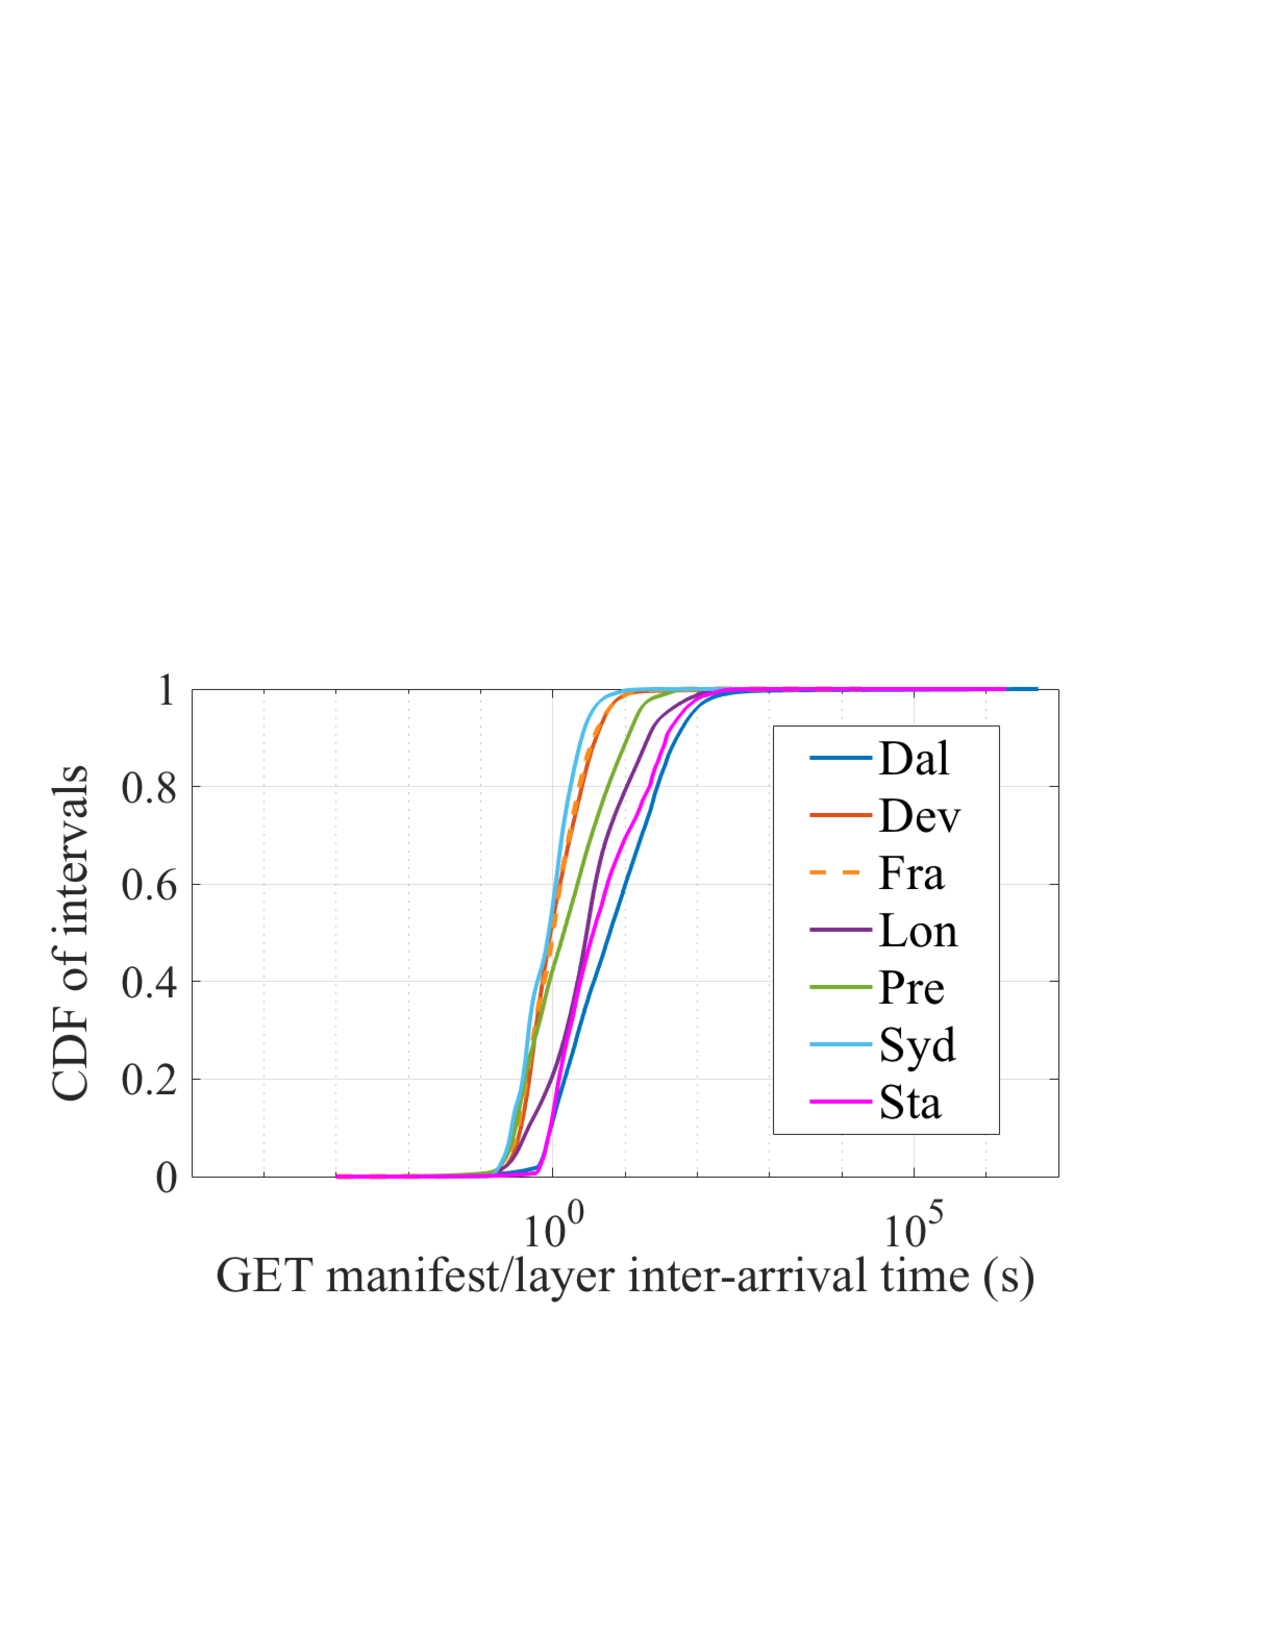
\includegraphics[width=0.3\textwidth]{graphs/GML-intervals.pdf}
	\caption{Intervals between \texttt{pull} manifest request and \texttt{pull} layer request}
	%	\vspace{-3pt}
	\label{fig:intervals}
	
\end{figure}
%\begin{figure*}[!t]
%	\centering
%	\subfigure[Layer repull count]{
%		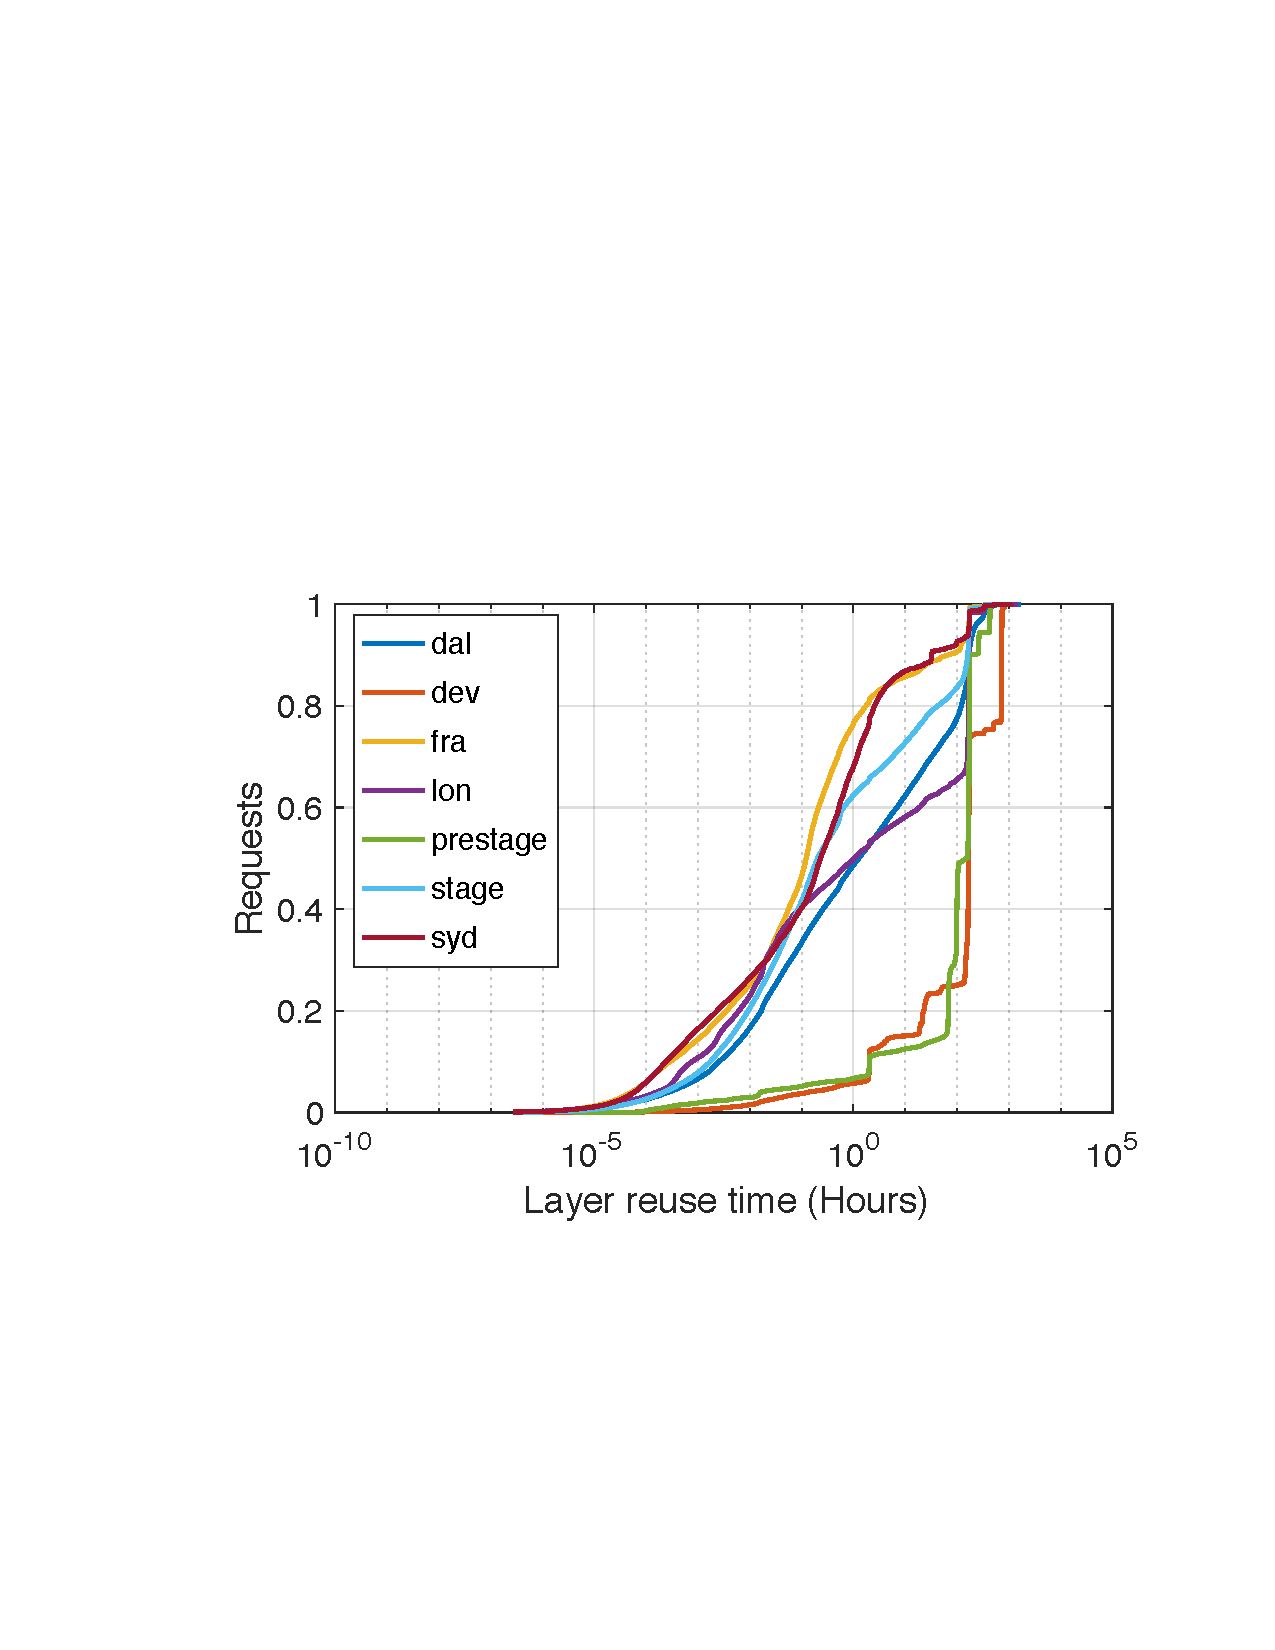
\includegraphics[width=0.2\linewidth]{graphs/layer-reusetime.pdf}
%			\label{fig:layer-reuse}
%	}
%	\subfigure[Repository repulling probability]{
%		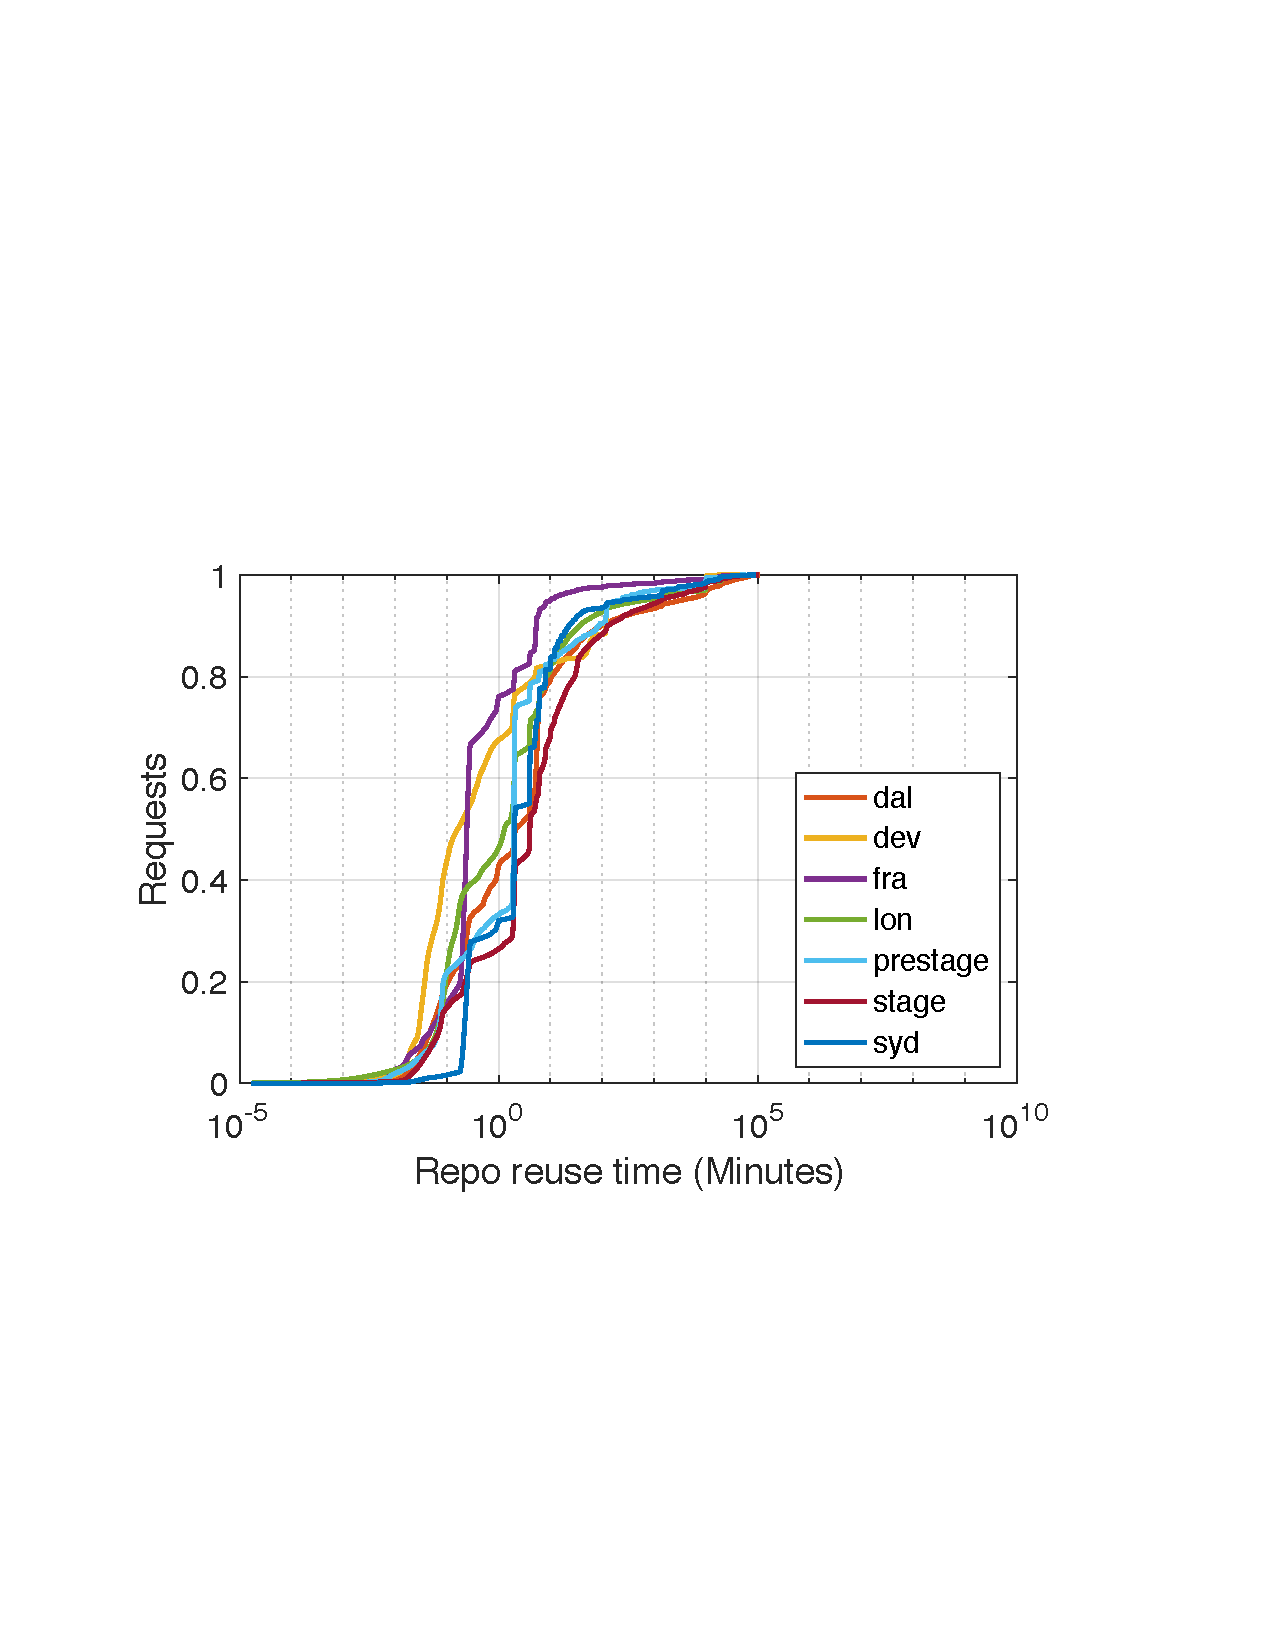
\includegraphics[width=0.2\linewidth]{graphs/repo-reusetime.pdf}
%				\label{fig:repo-reuse}
%	}
%	\subfigure[Client repulling probability]{
%		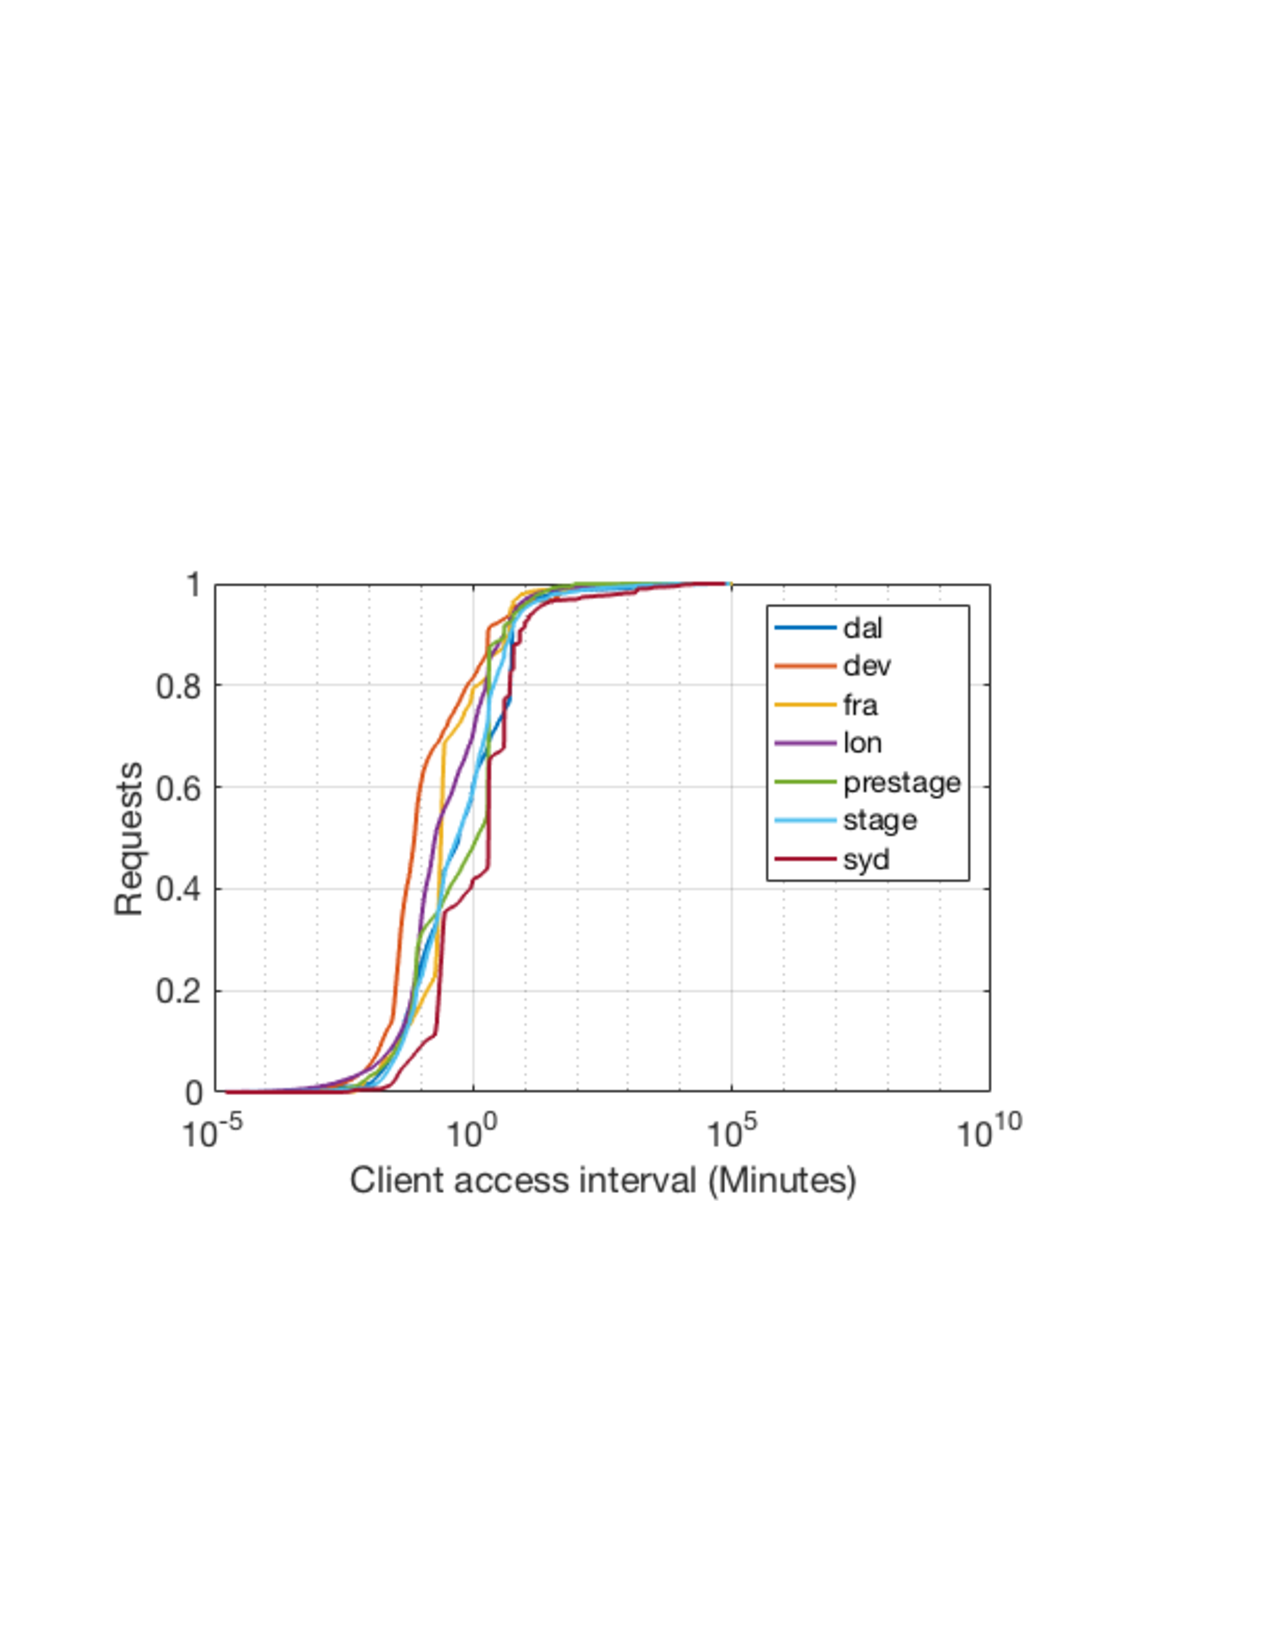
\includegraphics[width=0.2\linewidth]{graphs/user-intervals.pdf}
%			\label{fig:user-interval}
%	}
%	\caption{CDF of reusetime for layers, repositories and clients' access intervals.}
%	\label{fig:fig-reuse}
%\end{figure*}

%\begin{figure}[t]
%	\centering
%	\begin{minipage}{0.26\textwidth}
%		\centering
%		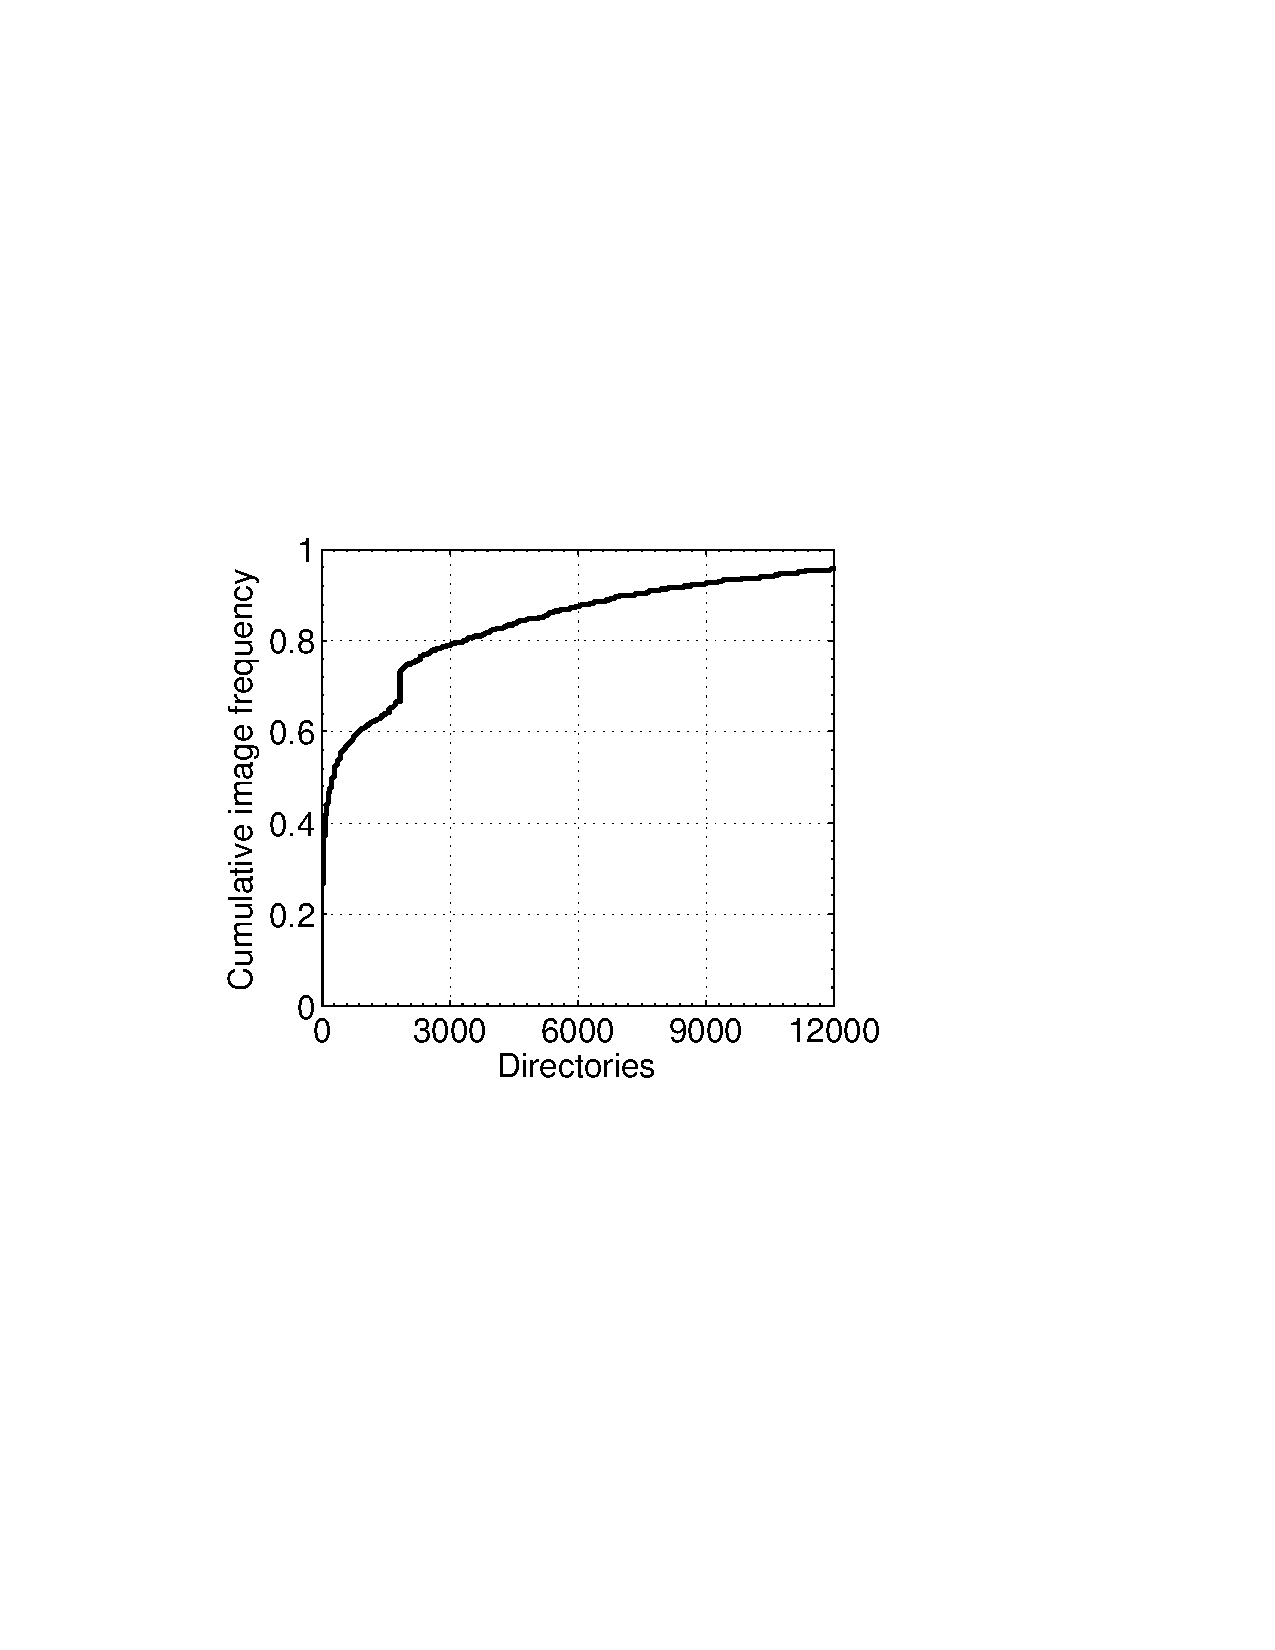
\includegraphics[width=1\textwidth]{graphs/dir.pdf}
%		\caption{CDF of images by\newline directories}
%		\label{fig-dir}
%	\end{minipage}%
%	\begin{minipage}{0.24\textwidth}
%		\centering
%		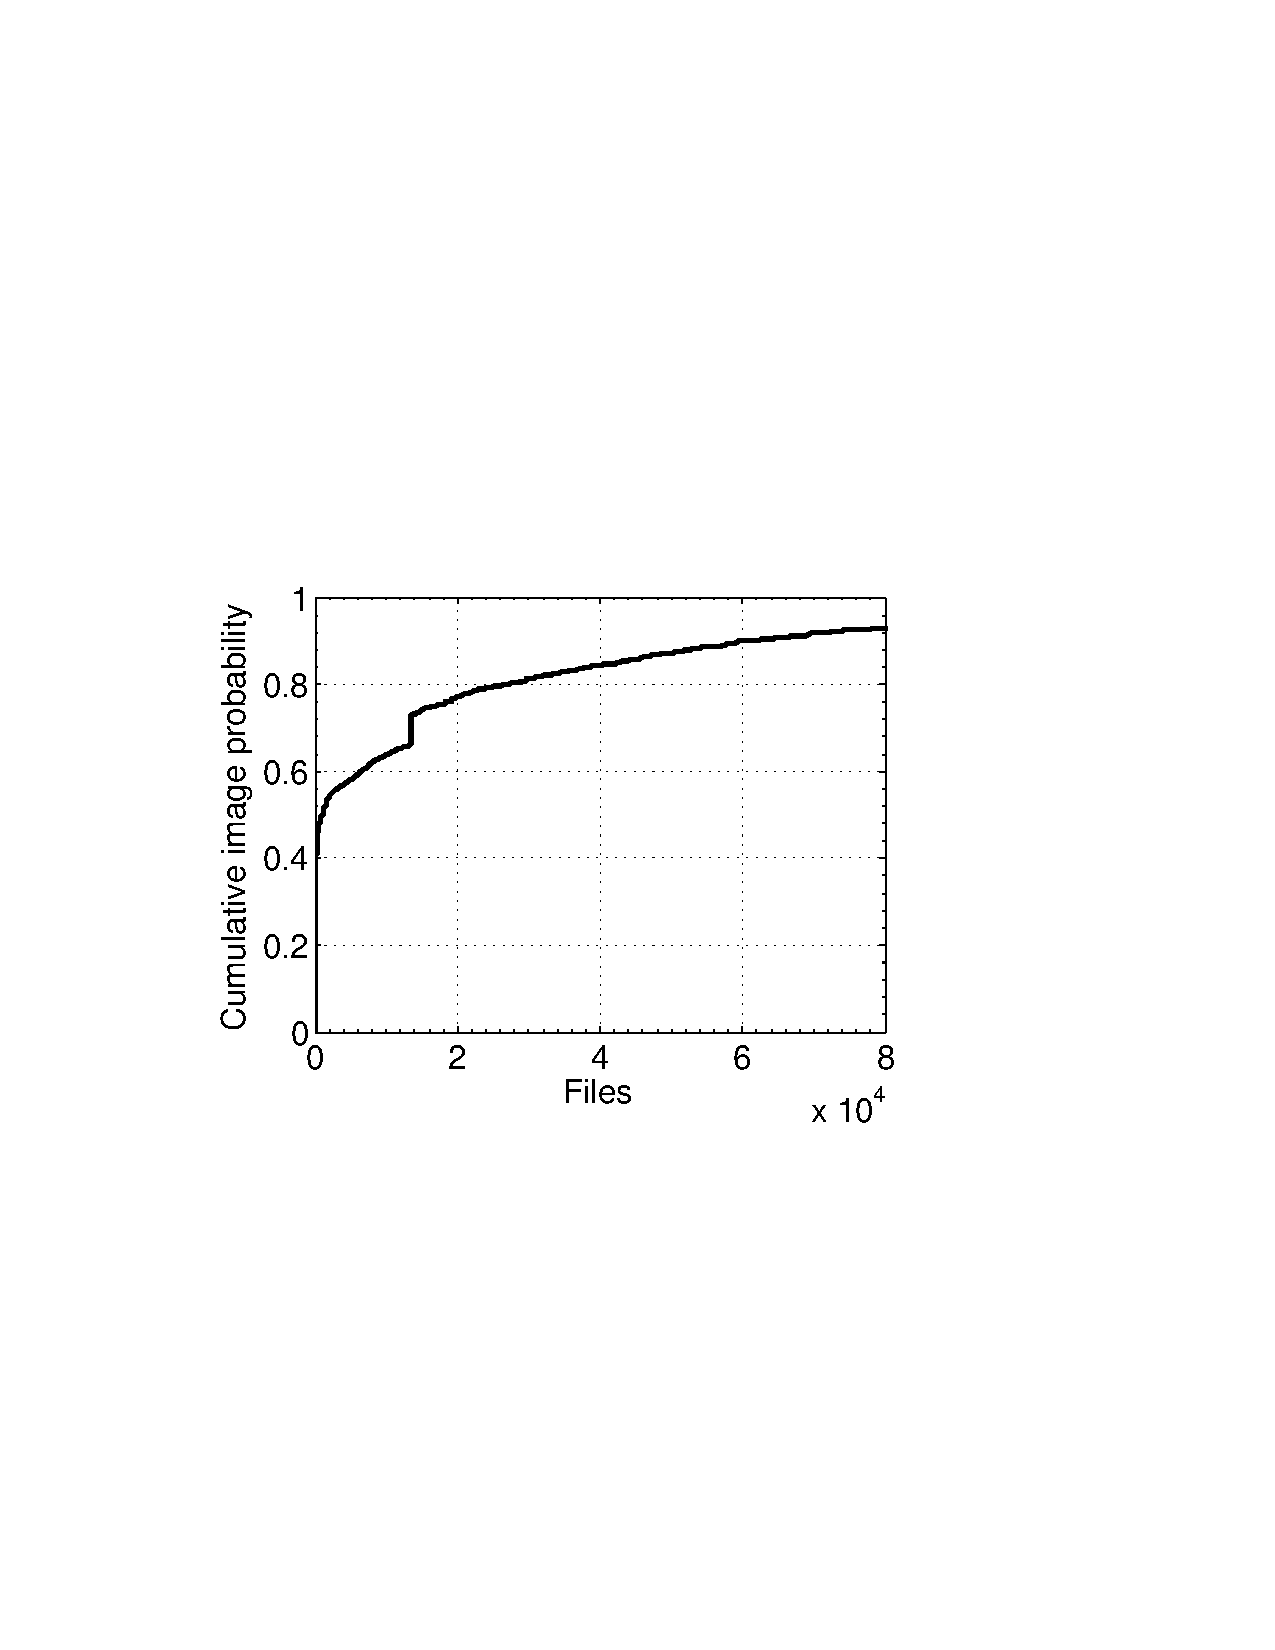
\includegraphics[width=1\textwidth]{graphs/file.pdf}
%		\caption{CDF of images by files}
%		\label{fig-file}
%	\end{minipage}
%\end{figure}

%\begin{figure}[htbp] 
%	\begin{minipage}{0.5\linewidth} 
%		\centering 
%		\includegraphics{circle} 
%		\caption{A Circle} 
%		\label{fig:circle} 
%	\end{minipage}% 
%	\begin{minipage}{0.5\linewidth} 
%		\centering 
%		\includegraphics{rectangle} 
%		\caption{A Rectangle} 
%		\label{fig:rectangle} 
%	\end{minipage} 
%\end{figure}

\preconstructcachename~starts cache eviction when free space is low.
To decide which layer or slices need to be evicted to make space for new requests,
we analyze the temporal trend of user accesses as follows.

\paragraph{Temporal trend}
Figure~\ref{fig:layer-skenwess} shows the CDF of layer popularity.
We observe a heavy layer access skewness for \texttt{Fra}, \texttt{Syd}, \texttt{Dal}, \texttt{Stage}, 
and \texttt{Lon}.
We see that 80\%, 70\%, and 60\% of the \texttt{pull} layer requests access only 10\% of layers, 
for \texttt{Fra}, \texttt{Syd}, \texttt{Dal}, \texttt{Stage}, 
and \texttt{Lon} respectively.
Figure~\ref{fig:repo-skewness} shows the CDF of repository popularity.
Compare to layer popularity, 
repository access skewness is heavier acorss 7 workloads.
Almost 90\% of \texttt{pull} layer requests access only 10\% of repositories for 
\texttt{Dev}, \texttt{Fra}, \texttt{Prestage}, \texttt{Syd}, and \texttt{Stage} respectively.
Almost 75\% of \texttt{pull} layer requests access only 10\% of repositories for
both \texttt{Dal} and \texttt{Lon}.
Figure~\ref{fig:client-skewness} shows the CDF of client popularity.
\texttt{Dal}, \texttt{Dev}, \texttt{Fra}, \texttt{Lon}, \texttt{Prestage}, and \texttt{Stage}
shows a heavey client access skewness.
10\% of clients send 95\% \texttt{pull} layer requests for \texttt{Lon}.
\texttt{Syd} shows a slight client skewness. 70\% of requests are sent by 36\% of clients.
Overall, caching a layer with higher pull count will improve the hit ratio, 
especially for popular repositories and active clients with higher repulling probability. 

Next, we analyze the layer and repository reuse time.
layer reuse time means the duration between two consecutive requests to the same layer
while repository reuse time means the duration between two consecutive \emph{pull} manifest requests to the same repository.
Figure~\ref{fig:layer-reuse} shows the CDF of layer reuse time. 
%Layer reuse time means the duration between two consecutive \texttt{pull} requests to the same layer.
We see that layer reuse time distribution varies among different workloads.
For \texttt{Fra}, \texttt{Syd}, and \texttt{Stage},
half of the layers' reuse time is shorter than 6 minutes.
While half of layers from \texttt{Dal} and \texttt{Lon} have a reuse time higher than 1 hour.
Half of layers from both \texttt{Prestage} and \texttt{Dev} are not accessed for over 100 hours.
Consequently, for \texttt{Dal}, \texttt{Lon}, \texttt{Prestage}, and \texttt{Dev}, 
it may take longer than 1 hour for at lease half newly requested layer to get a hit. 
These layers or the slices for them are unnecessarily for caching since 
their reuse time is too long and may cause other useful layers or slices to be evicted, called \emph{cache pollution}.
%Consider popular skewness, 
Figure~\ref{fig:repo-reuse} shows the CDF of repository reuse time.
%Repository reuse time means the duration between two consecutive \texttt{pull manifest} requests to the same repository.
We see that repository reuse time is much shorter than layer reuse time.
80\% of repositories are requested within 2-12 minutes across the 7 workloads.
Figure~\ref{fig:user-interval} shows the CDF of client access intervals.
client access interval means the duration between two consective requests issued by the same client.
Client access intervals are much shorter than repository reuse time.
80\% of client are active within 1 - 3 minutes for the 7 workloads. 
Hence, to eliminate \emph{cache pollution},
we consider the reuse time of layer and repository as well as client access intervals during
cache eviction.

\paragraph{Eviction algorithm}
As shown in algorithm~\ref{alg:eviction}, to exploit the temporal trend of clients and repositories, 
\preconstructcachename~set timers for its hosted layers, clients, and repositories.
Timeout happens when a layer along with its associated clients and repositories are all timeout.
\preconstructcachename~will remove this layer from cache.
Beside,
\preconstructcachename~maintains a LFRU list of cached layers~\cite{xxx} to exploit layer temporal trend.
If free space is low,
\preconstructcachename~selects the least frequent recently used layer which has a lower repulling probability to evict.



\begin{algorithm}
	\scriptsize 
	\caption{User access history based eviction.}
	\label{alg:eviction}
	\SetAlgoLined
	\KwIn{\\
		$T_{mem}$: Capacity threshold for MEM cache to trigger demotion. \\
		$T_{flash}$: Capacity threshold for FLASH cache to trigger eviction. \\
		$UsrLRU$: LRU of users.  \\
		$LayerLRU[Usr]$: LRU of layers that are accessed by user $Usr$. \\
		$RepoLRU$: LRU of repostiories. \\
		$LayerLRU[Repo]$: LRU of layers that are associated with repository $Repo$.
	}
	\While{free\_MEM $<$ $T_{mem}$}{
		\emph{last\_usr} $\gets$ \emph{UsrLRU.last\_item()}\\
		\For{last\_layer $\gets$ \emph{LayerLRU[last\_usr].last\_item()}}{
			\If{layer exclusively belongs to last\_usr}{
				%{\scriptsize $/*$\textit{If layer is not shared with other users, layer is deleted}}\\
			%	last\_layer $\gets$ \emph{LayerLRU[last\_usr]}\\			
				FLASHcache $\gets$ \emph{Demote(last\_layer)} \\
				\emph{free\_MEM} $+=$ \emph{sizeof(last\_layer)} \\
			}
		}
	}

	\While{free\_FLASH $<$ $T_{flash}$}{
	\emph{last\_repo} $\gets$ \emph{RepoLRU.last\_item()}\\
	\For{last\_layer $\gets$ \emph{LayerLRU[last\_repo].last\_item()}}{
		\If{layer exclusively belongs to last\_repo}{
			%{\scriptsize $/*$\textit{If layer is not shared with other users, layer is deleted}}\\
			%	last\_layer $\gets$ \emph{LayerLRU[last\_usr]}\\			
			\emph{Discard(last\_layer)} \\
			\emph{free\_FLASH} $+=$ \emph{sizeof(last\_layer)} \\
		}
	}
}

\end{algorithm}


%\begin{algorithm}
%    \tiny 
%	\caption{User access history based eviction}
%	\label{alg:prefetch}
%	%\SetAlgoLined
%	\KwIn{\\
%		$L_{thresh}$: Threshold for duration to keep a prefetched layer. \\
%		$RLMap$: Repository to layers map.\\
%		$URLMap$: User to layers map. \\
%	}
%	\While{true}{
%		\emph{r} $\leftarrow$ \texttt{request received}\\
%		\uIf{r = GET manifest}
%		{
%%			layerlst $\leftarrow$ URLMap[(r.client, r.repo)]
%			\emph{layers} $\gets$ \emph{RLMap[r.repo]} $-$ \emph{URLMap[r.client]} \\
%			\emph{OnTimelayers}, \emph{NotOnTimelayers} $\gets$ \emph{OnTimeCalculation(layers)} \\
%			\emph{MEMcache} $\gets$ \emph{Prefetch(OnTimelayers)} \\
%			\emph{FLASHcache} $\gets$ \emph{Prefetch(NotOnTimelayers)} \\
%			\texttt{set} \emph{L\_timer[layer] for each layer in layer} \\
%			{\tiny\texttt{/*when $L\_timer[layer] > L\_thresh$, layer is evicted/}}
%			}
%		\uElseIf{r = PUT layer }
%		{
%				\texttt{update} \emph{URLMap[(r.client, r.layer)]} \\
%				\texttt{update} \emph{RLMap[(r.repo, r.layer, put)]} \\
%				\emph{MEMcache} $\leftarrow$ \texttt{buffer} \emph{r.layer} \\
%				\texttt{set} \emph{L\_PUT\_timer[r.layer]} \\
%				{\tiny\texttt{/*when $L\_timer[layer] > L\_thresh$, layer is evicted/}}	 \\
%			}
%		\ElseIf{r = GET layer}
%		{
%				\eIf{r.layer in MEMcache or r.layer in FLASHcache}
%				{
%					\emph{serve from MEMcache or FLASHcache} \\
%					\texttt{update} \emph{URLMap[(r.client, r.layer)]} \\
%					\texttt{Reset} \emph{L\_timer[r.layer]}\\
%					\emph{hit++} 
%				}
%			   {
%					\emph{serve from backend storage system} \\
%					\texttt{update} \emph{URLMap[(r.client, r.layer, repulled)]} \\
%					\emph{RepulledLayers} $\gets$ \emph{RLMap[r.repo]} \\
%					\emph{FLASHcache} $\gets$ \emph{Prefetch(RepulledLayers)} \\
%					\texttt{set} \emph{L\_timer[layer] for each layer in layers} \\
%					{\tiny\texttt{/*when $L\_timer[layer] > L\_thresh$, layer is evicted/}}
%			}
%		}
%	}
%\end{algorithm}

